\hypertarget{ux7edfux4e00ux67b6ux6784ux7684ux591aux6a21ux6001ux7406ux89e3-ux751fux6210ux6a21ux578b}{%
\chapter{统一架构的多模态理解-生成模型}\label{ux7edfux4e00ux67b6ux6784ux7684ux591aux6a21ux6001ux7406ux89e3-ux751fux6210ux6a21ux578b}}

\hypertarget{ux591aux6a21ux6001ux7edfux4e00ux7406ux89e3-ux751fux6210ux6a21ux578bux6982ux8ff0}{%
\section{多模态统一理解-生成模型概述}\label{ux591aux6a21ux6001ux7edfux4e00ux7406ux89e3-ux751fux6210ux6a21ux578bux6982ux8ff0}}

\hypertarget{ux4e00ux57faux672cux4ecbux7ecd}{%
\subsection{一、基本介绍}\label{ux4e00ux57faux672cux4ecbux7ecd}}

多模态统一理解-生成模型将语言模型和生成模型/世界模型统一起来，前者处理表征人类逻辑的语言模态，后者处理其他表示世界客观状态的模态。这样，模型既具备了LLM的逻辑推理能力，又具备了对世界的物理认知和规划能力，在没有明显能力短板的情况下根据The Bitter Lesson将可以随着规模扩展而不断提升，乃至涌现出更高级的融合能力。

当然，不是所有目前的多模态统一理解-生成模型都具备世界模型的预测下一状态能力。智源Emu支持世界模型的预测；LongCat-Next能生图、理论上架构可以用于状态预测，但没有按世界模型训练，没有建模跨帧token依赖，没有引入时序压缩或帧间残差编码，没有视频数据预训练；Transfusion没有世界模型能力，静态图像在diffusion生成过程中内部独立去噪，没有跨帧状态传递，联合建模困难；字节BAGEL虽然没有针对世界模型专门训练，但通过大规模图/视频/文本交错训练，涌现了一定的视觉建模能力。

\hypertarget{ux4e8cux6838ux5fc3ux96beux70b9ux4e0eux539fux56e0}{%
\subsection{二、核心难点与原因}\label{ux4e8cux6838ux5fc3ux96beux70b9ux4e0eux539fux56e0}}

在多模态统一理解-生成模型的训练中，最大的难题在于理解和生成的梯度常出现冲突，而不是形成有效的信息增益和相互促进。大体有以下几种解释。

\begin{enumerate}
\def\labelenumi{\arabic{enumi}.}
\item
  图像生成需要复杂的空间规划、物理常识和语义推理，模型在一次前向传播中能执行的逻辑推理步骤是有限的，导致梯度信号太粗糙，理解模型没法给生成模型有效指导，生成模块的失败也无法有效地帮助理解模块进步。可能需要引入CoT等。（阶跃星辰）
\item
  图像信息丰富，而单一有限的离散Token词表表征容量太小，结果只能要么丢失整体语义信息，要么丢失细节信息。（字节UniTok）
\item
  理解任务的逻辑是从具体到抽象的认知过程，生成任务的逻辑是从抽象到具体的重建过程。
\end{enumerate}

\hypertarget{ux53c2ux8003ux6587ux732e-195}{%
\subsection{参考文献}\label{ux53c2ux8003ux6587ux732e-195}}

\begin{itemize}
\tightlist
\item
  Team Chameleon. (2024). \href{https://arxiv.org/abs/2405.09818}{Chameleon: Mixed-Modal Early-Fusion Foundation Models}. arXiv:2405.09818.
\item
  Xie, J., Mao, W., Bai, Z., Zhang, D. J., Wang, W., Lin, K. Q., Gu, Y., Chen, Z., Yang, Z., \& Shou, M. Z. (2024). \href{https://arxiv.org/abs/2408.12528}{Show-o: One Single Transformer to Unify Multimodal Understanding and Generation}. arXiv:2408.12528.
\item
  Wu, C., Chen, X., Wu, Z., Ma, Y., Liu, X., Pan, Z., Liu, W., Xie, Z., Yu, X., Ruan, C., \& Luo, P. (2024). \href{https://arxiv.org/abs/2410.13848}{Janus: Decoupling Visual Encoding for Unified Multimodal Understanding and Generation}. arXiv:2410.13848.
\end{itemize}

\clearpage

\hypertarget{ux591aux6a21ux6001ux7edfux4e00ux7406ux89e3-ux751fux6210ux6a21ux578bux7684ux8f93ux5165ux7f16ux7801ux8bbaux6587}{%
\section{多模态统一理解-生成模型的输入编码（论文）}\label{ux591aux6a21ux6001ux7edfux4e00ux7406ux89e3-ux751fux6210ux6a21ux578bux7684ux8f93ux5165ux7f16ux7801ux8bbaux6587}}

\begin{quote}
本文是论文阅读笔记，内容代表对应论文方法或作者理解，不应直接视为领域共识或工程最佳实践。
\end{quote}

\hypertarget{ux4e00ux4e3bux8981ux7f16ux7801ux65b9ux6848}{%
\subsection{一、主要编码方案}\label{ux4e00ux4e3bux8981ux7f16ux7801ux65b9ux6848}}

对于图像等连续模态，如果像 LLM 一样直接离散编码，将出现问题：图像信息密度高，直接离散化会导致 Codebook 极其庞大；用于理解的整体语义信息和用于生成的局部信息容易出现冲突，难以取得平衡。为此，出现了一些主要的输入编码处理路线。

\hypertarget{ux4e00ux79bbux6563ux7f16ux7801ux7406ux89e3ux751fux6210ux5408ux6d41ux7f16ux7801ux667aux6e90-emulongcat-nextux5b57ux8282-unitok}{%
\subsubsection{（一）离散编码+理解生成合流编码（智源 Emu、LongCat-Next、字节 UniTok）}\label{ux4e00ux79bbux6563ux7f16ux7801ux7406ux89e3ux751fux6210ux5408ux6d41ux7f16ux7801ux667aux6e90-emulongcat-nextux5b57ux8282-unitok}}

这种方案下，一般将图像转化为离散的 token IDs，以适配目前通用的自回归模型架构。

为了让模型能像处理文本一样处理图像，系统底层包含一个视觉分词器（通常是基于 VQ-VAE 架构）。它的作用是将连续的图像像素空间进行压缩、量化，并映射到一个离散的``视觉词表''中。这样一来，图像就被切分成了一系列离散的视觉标记（Visual Tokens），它们在格式和维度上与文本标记（Text Tokens）实现了平权。

LongCat-Next 论文指出，通过增加训练数据，离散表征可以无限逼近连续表征的效果。运用离散表征的好处在于两方面：首先，可以使得图像等模态与 LLM 的 Next token prediction 完成统一；其次，与 GRPO 等强化学习方法天然兼容，不用像流匹配模型那样为了能进行 RL 而专门从 ODE 改为 SDE。

但是核心难点在于，单一有限的离散 Token 词表表征容量太小。有一些解决方法：

\begin{enumerate}
\def\labelenumi{\arabic{enumi}.}
\tightlist
\item
  分块、分层 Codebook（LongCat-Next）：模型不使用一本``大词典''，而是用 8*K（K 为一张图的分块数）本``分层词典''，将它们的结果组合起来。这就类似于计算机中，只要用 14 位 0 或 1 的二进制数组合起来，就可以表征 16384 种组合。
\end{enumerate}

一张图像先分为若干块，然后对于每一个图像块，在经过 VQ-VAE 后，通过残差向量量化的方式切分 token（注意残差向量量化这一步没有参数，而是硬编码取词表中匹配度最高者，词表的 Embedding 向量值是和主模型一起训练的）。

\begin{itemize}
\tightlist
\item
  \textbf{Level 1（\(l=1\)）}：首先，模型尝试用第一层密码本去匹配原始图像特征。这第一层捕捉的是最核心、最抽象的语义信息（比如``这是一只猫的耳朵''）。
\item
  \textbf{计算残差}：第一层的匹配必然不够精确，会产生误差（残差 = 原始特征 - 第一层特征）。
\item
  \textbf{Level 2（\(l=2\)）}：接着，模型用第二层密码本去专门量化这个``残差''。第二层捕捉的是次一级的细节。
\item
  \textbf{循环往复}：以此类推，直到第 8 层（\(l=8\)）。每一层都在修补上一层留下的微小误差，捕捉越来越精细的高频纹理和边缘信息。
\end{itemize}

这 8 个层级的向量都有各自的词表空间，分别记录从整体到局部的特征，它们通过加法融合，整体特征更多服务于理解，局部特征更多服务于生成，事实上巧妙地解决了冲突问题。

值得注意的是，消融实验发现多级 embedding 加和后若不重新编码，性能会下降。为此引入单层 FFN，在 Codebook lookup 后对加和特征重新映射，防止多级信息叠加后语义坍缩。

\begin{enumerate}
\def\labelenumi{\arabic{enumi}.}
\setcounter{enumi}{1}
\tightlist
\item
  二进制 Codebook（UniWeTok）：在传统的 VQ-VAE 或 VQGAN 中，Codebook 是一个显式存在的可学习参数矩阵。编码器输出下一个向量时，需要和其中所有向量计算距离并取最小。图像信息丰富，需要 Codebook 容量极大，会导致距离计算成本极高。可以采用二值化方法，利用向量每一个维度的正负号构建 Codebook，为正就量化为 1，为负就量化为 -1，构建了一个大小为 \(2^{d_{\mathrm{model}}}\) 的 Codebook。
\end{enumerate}

\hypertarget{ux4e8cux79bbux6563ux7f16ux7801ux7406ux89e3ux751fux6210ux5206ux5f00ux7f16ux7801deepseek-janus}{%
\subsubsection{（二）离散编码+理解生成分开编码（DeepSeek Janus）}\label{ux4e8cux79bbux6563ux7f16ux7801ux7406ux89e3ux751fux6210ux5206ux5f00ux7f16ux7801deepseek-janus}}

我们知道，理解和生成任务在同一个编码器中的梯度冲突很可能是因为需要的信息类型不同。因此，一个直观的方法是用不同的编码器分开编码：理解型编码器输出的编码更多服务于文本生成；生成型编码器输出的编码更多服务于视觉生成。

纯自回归的 Janus 在理解用 CLIP/SigLIP，生成用 VQ tokenizer。Janus 在理解任务中只启用理解型编码器，反之亦然。

\hypertarget{ux4e09ux8fdeux7eedux7f16ux7801ux7406ux89e3ux751fux6210ux5206ux5f00ux7f16ux7801ux5b57ux8282-bagelmeta-transfusion}{%
\subsubsection{（三）连续编码+理解生成分开编码（字节 BAGEL、Meta Transfusion）}\label{ux4e09ux8fdeux7eedux7f16ux7801ux7406ux89e3ux751fux6210ux5206ux5f00ux7f16ux7801ux5b57ux8282-bagelmeta-transfusion}}

\begin{itemize}
\tightlist
\item
  \textbf{文本输入}：直接通过语言模型自带的 Embedding 层（词表查找），转化为文本 Token（\(X_{\mathrm{text}}\)）。
\item
  \textbf{图像输入}：这张原始图片（像素矩阵）会被同时复制两份，分别喂给两个视觉编码器：

  \begin{itemize}
  \tightlist
  \item
    喂给 ViT，输出代表高级概念的语义 Token（\(X_{\mathrm{ViT}}\)）。
  \item
    喂给 VAE Encoder，输出代表连续空间结构的隐变量 Token（\(X_{\mathrm{VAE}}\)）。
  \end{itemize}
\end{itemize}

不同于 Janus 在理解任务中只启用理解型编码器（反之亦然），BAGEL 为了更好地统一理解与生成任务，将三种 Token 被拼接为序列，一起输入一个统一的自注意力层。当模型准备开始生成图像时，会在自注意力层后面接一个 \texttt{{[}BOI{]}} token，并在后面注入一定数量（如 1024 个）噪声 token（训练时为目标图像加噪得到，测试时则直接采样白噪声），开始并行去噪、预测流速度。

若 VAE 编码结果的向量维度仍然大于 Transformer 的输入向量维度，可以用线性池化下采样或 U-Net 下采样方案。后者需要的参数量更大，但生成质量更高。

Janus 和 BAEGL 论文的实验均证明，共用编码器时，加入生成任务后，模型理解指标明显下降，CE loss 上升，说明共享表征时生成会挤占理解的语义容量，二者存在强烈冲突；解耦架构实验（双专家+双编码器）中，生成任务不再破坏理解性能，同时理解特征能为生成提供语义约束，让图像更贴合文本、细节更准确，实现理解与生成双向协同。

\hypertarget{ux56dbux8fdeux7eedux7f16ux7801ux7406ux89e3ux751fux6210ux5408ux6d41ux7f16ux7801rae}{%
\subsubsection{（四）连续编码+理解生成合流编码（RAE）}\label{ux56dbux8fdeux7eedux7f16ux7801ux7406ux89e3ux751fux6210ux5408ux6d41ux7f16ux7801rae}}

在过去的统一多模态模型中，``看''和``画''实际上使用的是两套完全不同的特征语言：

\begin{itemize}
\item
  \textbf{视觉理解（看）}：大语言模型（LLM）为了看懂图片，通常会使用 CLIP 或 SigLIP 这样的表征编码器。这些编码器提取出来的是高维的、富含语义的特征（例如 1152 维）。这就像是 LLM 的``视觉母语''。
\item
  \textbf{视觉生成（画）}：传统的扩散模型为了节省算力，使用 VAE 将像素极度压缩成低维的隐特征（例如几十维），在这个低维空间里进行去噪生成。
\item
  \textbf{分裂的痛点}：因为扩散模型生成的是 VAE 低维特征，而 LLM 只认识 CLIP/SigLIP 的高维语义特征。如果扩散模型画完一张草稿（VAE 隐特征），LLM 是完全看不懂的。
\item
  \textbf{传统工作流}：如果 LLM 想检查扩散模型画得对不对，必须经过极其繁琐的步骤：扩散模型生成 VAE 特征 -\textgreater{} VAE 解码器将其还原为像素图片 -\textgreater{} CLIP 编码器重新将像素图片编码为高维特征 -\textgreater{} LLM 进行评估。这就导致模型仿佛有两个不互通的大脑。
\end{itemize}

RAE 的核心思想非常直接：既然 LLM 习惯看 SigLIP 的高维语义特征，那我们为什么不逼着扩散模型直接去生成 SigLIP 的高维语义特征呢？

所以，在 RAE 的架构下，它并没有取消编码器，而是彻底抛弃了 VAE 编码器，统一只使用 SigLIP-2 作为唯一的编码器。

\begin{itemize}
\tightlist
\item
  \textbf{统一的生成空间}：扩散模型不再预测 VAE 的低维特征，而是直接在 \(16\times16\times1152\) 维的 SigLIP-2 语义特征空间里进行去噪生成。
\item
  \textbf{无缝的模态互通}：因为扩散模型生成的直接就是 SigLIP-2 特征，这恰好是 LLM 的``母语''。这意味着，扩散模型刚在隐空间里把事情打好，LLM 不需要经过任何像素解码和重新编码，直接就能读取这些特征序列，立刻判断出这张图画得符不符合要求。
\end{itemize}

此外，过去的理解-生成统一模型常为了迁就生成任务的算力而使用低维压缩表征，无法同时满足理解所需的语义容量与生成所需的细节精度，正是引起两种任务发生冲突的重要原因。

不同于 VAE 编码器、解码器参数量相等，RAE 采取重编码器、轻解码器的方法：

\begin{itemize}
\tightlist
\item
  \textbf{重编码器（Heavy Encoder）}：直接``白嫖''开源的、参数量极其庞大的视觉基础模型（Foundation Model，例如数十亿参数的 SigLIP-2、DINOv2 或 MAE）。它的任务是深思熟虑地``看透''真实图像，提取出极其高维、富含语义的特征表示。
\item
  \textbf{轻解码器（Light Decoder）}：仅仅是一个层数很少、参数量极小的浅层 ViT（Vision Transformer）。因为重编码器提取的特征已经包含了完美的信息，解码器不需要再进行复杂的语义推理，它只负责做一个简单的``翻译工''------将高维特征矩阵``降维打击''成人类肉眼可见的 RGB 像素矩阵。
\end{itemize}

由于在高维空间内扩散生成较费算力，轻解码器恰恰减轻了算力负担，起到了平衡作用。（生成图像时不需要编码器）

总结来说：RAE 不是回到了低级的像素空间，而是把``生成''这件事，强行拉升到了和``理解''同一个级别的高维语义空间。

随规模扩展，加宽扩散头、噪声增强解码等机制几乎不再带来收益。但部分机制必须保留：

\begin{itemize}
\tightlist
\item
  \textbf{必须保留的核心机制：维度感知噪声调度（Dimension-aware noise scheduling）}。因为高维空间与低维空间特性不同，必须根据有效数据维度 \(m\)（Token 数乘以特征维度）对时间步进行偏移缩放。去掉该机制会导致模型性能灾难性下降。时间步偏移公式为：
\end{itemize}

\[
t_m=\frac{\alpha t_n}{1+(\alpha-1)t_n}
\]

其中 \(n\) 为基准维度，\(\alpha=\frac{m}{n}\)。

此外，RAE 比 VAE 更能有效避免过拟合：

在现代 T2I 模型的``大规模预训练 + 高质量小数据微调''范式中，过拟合是一个致命问题。

\begin{itemize}
\tightlist
\item
  \textbf{VAE 的脆弱}：实验观察到，基于 VAE 的模型在高质量数据集上微调仅仅 64 个 Epoch 后，就会遭遇灾难性的过拟合。它的训练损失会迅速暴跌，模型开始死记硬背训练样本，丧失泛化能力。
\item
  \textbf{RAE 的稳定}：相反，RAE 模型展现出了惊人的稳定性。即使微调到长到 256 个 Epoch 甚至 512 个 Epoch，它的性能依然保持坚挺。论文推测，RAE 的高维且高度语义化的隐空间起到了``隐式正则化''的作用，强迫模型学习真正的特征分布，而不是死记硬背像素细节。
\end{itemize}

后续研究：Beyond Language Modeling 表明，高维 RAE 表征可同时提升生成与理解性能，传统范式中``LLM 主导、视觉从属''嫁接架构是导致二者难以协同的核心原因，因为该范式会迫使视觉表征向文本对齐，进而牺牲理解细粒度或生成精准度，加剧模态冲突。该工作的核心实验围绕生成与理解的双向促进关系展开，采用统一 Transformer 架构搭配 RAE 表征，在纯文本、纯视频、图像-文本对、动作视频的混合数据上从零预训练。实验及结论：

\begin{enumerate}
\def\labelenumi{\arabic{enumi}.}
\tightlist
\item
  双向增益实验：固定视觉 token 预算，增加文本 token 可持续提升生成质量；固定文本 token 预算，增加视觉 token 不损害语言建模效果，证明视觉与语言任务无负向冲突；
\item
  泛化增益实验：20B VQA 数据搭配 80B 通用多模态数据（视频/图像-文本/文本），VQA 效果超越 100B 纯 VQA 数据训练结果，证实生成相关多模态数据可反哺视觉理解能力；
\item
  范式对比实验：原生多模态联合预训练显著优于 LLM 嫁接视觉的范式，在理解与生成任务上全面领先，证明平等模态架构是释放双向增益的关键。
\end{enumerate}

\hypertarget{ux4e8cembedding-ux8badux7ec3ux65b9ux6cd5}{%
\subsection{二、Embedding 训练方法}\label{ux4e8cembedding-ux8badux7ec3ux65b9ux6cd5}}

需要说明的是，下面不同的损失常配合使用。

\hypertarget{ux4e00ux5bf9ux6bd4ux5b66ux4e60-1}{%
\subsubsection{（一）对比学习}\label{ux4e00ux5bf9ux6bd4ux5b66ux4e60-1}}

主流视觉编码器（SigLIP、CLIP 等）采用的方法，拉近图像全局特征与文本特征的距离。

\[
\mathcal{L}_{\mathrm{contrastive}}
=-\log\frac{\exp(s(I,T)/\tau)}
{\sum_j\exp(s(I,T_j)/\tau)}
\]

这种方式能实现高层语义对齐，但会丢失细节，无法用于生成。

\hypertarget{ux4e8cux91cdux5efaux635fux5931}{%
\subsubsection{（二）重建损失}\label{ux4e8cux91cdux5efaux635fux5931}}

为了避免丢失细节信息，可用类似于 VAE Loss，含 MSE、感知损失（用预训练神经网络提取特征后计算相似度）和 GAN 损失。中科院、MEGVII 和面壁智能的 ROSS 通过实验指出，重建损失能提升理解能力，文生图则不一定，因为前者梯度精细、稳定。

\hypertarget{ux4e09ux539fux751fux591aux6a21ux6001ux9884ux8badux7ec3}{%
\subsubsection{（三）原生多模态预训练}\label{ux4e09ux539fux751fux591aux6a21ux6001ux9884ux8badux7ec3}}

如果从零进行主模型的预训练，可以在训练中引入各种视觉整体、细节理解和生成任务，让编码器自主学习到既保留高层语义，又保留底层细节的编码方式。

另外，对于不同分辨率的图像，可以用自适应分辨率方法，或先在固定分辨率预训练，后续微调时让模型适应不同分辨率。人脸数据和文字图像等可精调。

\hypertarget{ux4e09ux79bbux6563ux7f16ux7801ux65b9ux6848ux4e2dux7684ux7279ux6b8aux8badux7ec3ux65b9ux6cd5}{%
\subsection{三、离散编码方案中的特殊训练方法}\label{ux4e09ux79bbux6563ux7f16ux7801ux65b9ux6848ux4e2dux7684ux7279ux6b8aux8badux7ec3ux65b9ux6cd5}}

\hypertarget{ux4e00ux5229ux7528ux8fdeux7eedux7f16ux7801ux5668ux8badux7ec3ux79bbux6563ux7f16ux7801ux5668}{%
\subsubsection{（一）利用连续编码器训练离散编码器}\label{ux4e00ux5229ux7528ux8fdeux7eedux7f16ux7801ux5668ux8badux7ec3ux79bbux6563ux7f16ux7801ux5668}}

事实上，离散编码器本身和连续编码器的区别仅仅就是在后面多了一个 Codebook 取近邻。故可以利用连续编码器，训练得到语义完备的连续编码器。具体方式包括：

\begin{enumerate}
\def\labelenumi{\arabic{enumi}.}
\tightlist
\item
  蒸馏连续编码器：让离散编码器蒸馏连续编码器的输出。通过余弦相似度损失，让每一层激活值接近连续编码器对应层激活值。
\end{enumerate}

对于离散 Codebook，UniWeTok 提出应同时在量化操作前和量化操作后蒸馏。量化后蒸馏是防止量化导致蒸馏到的信息丢失；量化前蒸馏是因为后面会提到我们强行让损失对码本离散向量的梯度变成了损失对编码器得到的连续向量的梯度，但实际上这两个梯度是不等的，只靠量化后蒸馏会导致回传的梯度不准。

\begin{enumerate}
\def\labelenumi{\arabic{enumi}.}
\setcounter{enumi}{1}
\tightlist
\item
  以连续编码器作为初始权重微调。
\end{enumerate}

\hypertarget{ux4e8cux79bbux6563ux5316ux65b9ux6848ux7684ux5176ux4ed6ux989dux5916ux635fux5931ux51fdux6570}{%
\subsubsection{（二）离散化方案的其他额外损失函数}\label{ux4e8cux79bbux6563ux5316ux65b9ux6848ux7684ux5176ux4ed6ux989dux5916ux635fux5931ux51fdux6570}}

\begin{enumerate}
\def\labelenumi{\arabic{enumi}.}
\tightlist
\item
  Commitment Loss
\end{enumerate}

\[
\alpha\lVert U_G-\mathrm{sg}[Q]\rVert^2
\]

\begin{itemize}
\tightlist
\item
  \textbf{含义}：\(U_G\) 是编码器输出的连续潜变量，\(Q\) 是离散化后的量化特征（来自密码本）。\(\mathrm{sg}[\cdot]\) 代表停止梯度（stop-gradient）操作。
\item
  \textbf{作用}：由于在量化过程中存在信息丢失，这个损失强迫编码器输出的连续特征 \(U_G\) 主动去``承诺''或``靠近''选定的离散特征 \(Q\)。这防止了连续特征在潜空间中随意游走，确保量化过程的稳定性。
\end{itemize}

\begin{enumerate}
\def\labelenumi{\arabic{enumi}.}
\setcounter{enumi}{1}
\tightlist
\item
  Entropy Loss
\end{enumerate}

这个损失分为两部分：Token Entropy Loss 要求模型在面对单个 token 时必须``极其果断''，不确定性越小越好；Codebook Entropy Loss 损失要求模型在面对全局数据时必须``雨露均沾''，不确定性适当大，以充分利用 Codebook，防止模型只利用少数 token。

\begin{enumerate}
\def\labelenumi{\arabic{enumi}.}
\setcounter{enumi}{2}
\tightlist
\item
  Generative-Aware Prior（GAP）
\end{enumerate}

可用一个轻量级的模型作为``代理生成器''，在 tokenizer 训练时就施加 next-token 对应图像生成的监督，迫使 token 的分布本身对自回归生成友好。

\hypertarget{ux4e09codebook-ux7684ux8badux7ec3ux95eeux9898ux4e0e-ste}{%
\subsubsection{（三）Codebook 的训练问题与 STE}\label{ux4e09codebook-ux7684ux8badux7ec3ux95eeux9898ux4e0e-ste}}

Codebook 中的向量用随机或聚类初始化。但在训练时，往往会碰到问题：

在 VQ 架构中，编码器输出连续向量 \(z_e\)，量化器通过查找码本输出离散的码本向量 \(z_q\)（即 \(e_k\)），最后解码器将 \(z_q\) 还原为图像。

这里的量化操作（找最近邻）在数学上表达为：

\[
k=\arg\min_j\lVert z_e-e_j\rVert_2
\]

\[
z_q=e_k
\]

梯度的灾难在于 \(\arg\min\) 函数的数学性质：它是一个分段的阶跃函数（Step Function）。如果你稍微改变一点点编码器的输出 \(z_e\)：

\begin{enumerate}
\def\labelenumi{\arabic{enumi}.}
\tightlist
\item
  大多数情况下，它离当前的 \(e_k\) 依然是最近的，选中的索引 \(k\) 不变，\(z_q\) 也不变。此时导数为 0。
\item
  极少数情况下，\(z_e\) 恰好跨过边界，索引 \(k\) 发生突变。此时导数为无穷大（\(\infty\)）。
\end{enumerate}

因此训练时会运用直通估计器（STE），对于编码器网络的连续输出 \(z_e\)，前向传播时离散编码器最终输出 \(z_q\) 会被赋值为 Codebook 里的 \(e_k\)，反向传播时则让损失对编码器最终输出 \(z_q\) 的梯度直接被替换为对连续输出 \(z_e\) 的梯度。公式为：

\[
z_q=z_e+\mathrm{sg}[e_k-z_e]
\]

结果：解码器传回来的梯度 \(\frac{\partial L}{\partial z_q}\)，不仅没有变成 0，反而以 1:1 的比例，毫发无损地``穿透''了量化层，直接交给了编码器。

但这样做的后果是，\(L\) 对码本向量 \(e_k\) 的梯度变成了 0，需要引入其他机制更新码本。一般有以下两种方法：

\textbf{机制 A：码本损失（Codebook Loss）------ 基于梯度的经典做法}

在总损失函数中，人为强制增加一项额外的惩罚项。

对于每次前向传播中被选中的码本向量 \(e_k\) 和对应的编码器连续特征 \(z_e\)，计算它们之间的均方误差（MSE）：

\[
\mathcal{L}_{\mathrm{codebook}}
=\lVert \mathrm{sg}[z_e]-e_k\rVert_2^2
\]

\begin{itemize}
\tightlist
\item
  \textbf{原理解释}：这里的 \(\mathrm{sg}[\cdot]\) 代表 Stop-Gradient（停止梯度）。这意味着在这个损失项中，我们把编码器的输出 \(z_e\) 当作一个``固定的目标锚点''。
\item
  \textbf{更新过程}：优化器在计算这个损失的梯度时，只会去更新码本向量 \(e_k\)，迫使它在连续空间中``一步步走向''编码器的输出 \(z_e\)。
\end{itemize}

注：同时为了防止编码器乱跑，还会有一个对应的 Commitment Loss \(\lVert z_e-\mathrm{sg}[e_k]\rVert_2^2\) 迫使编码器输出向码本靠拢，二者双向奔赴。

\textbf{机制 B：指数移动平均（EMA, Exponential Moving Average）------ 更稳定的现代做法}

在实际训练大规模 VQ-VAE 或 VQ-GAN（包括 UniTok 的底层）时，使用梯度下降更新码本往往非常不稳定。因此，现代架构更倾向于完全放弃使用优化器更新码本，而是采用 EMA。

\begin{itemize}
\tightlist
\item
  \textbf{更新过程}：
\end{itemize}

\begin{enumerate}
\def\labelenumi{\arabic{enumi}.}
\tightlist
\item
  在每个 Batch 中，记录下有哪些连续特征 \(z_e\) 被分配给了当前的码本向量 \(e_k\)。
\item
  计算这个 Batch 中分配给 \(e_k\) 的所有 \(z_e\) 的均值（假设记为 \(\bar z\)）。
\item
  直接用移动平均公式强行更新 \(e_k\) 的权重：
\end{enumerate}

\[
e_k^{(\mathrm{new})}
=\gamma\cdot e_k^{(\mathrm{old})}+(1-\gamma)\cdot\bar z
\]

其中 \(\gamma\) 是衰减系数，如 0.99。

\begin{itemize}
\tightlist
\item
  \textbf{优势}：EMA 更新不需要计算梯度，它就像是在动态地执行``在线 K-Means''，使得码本向量能非常平滑、稳定地追踪编码器特征分布的变化。
\end{itemize}

\textbf{机制 C：UniTok 的特殊更新（语义蒸馏注入）}

对于 UniTok 而言，除了上述的基础重构更新（让码本贴近图像特征），它的码本还承受着语义对齐的任务。

在 UniTok 的对比学习目标（如 Image-Text Contrastive Loss）中，被激活的离散 Token 对应的码本向量 \(e_k\)，会与对应的文本连续向量计算余弦相似度。这会产生额外的梯度，强迫码本向量 \(e_k\) 不仅要像原图的 Patch，还要在连续高维空间中移动到与文本描述对齐的位置。

此外，为保证 Codebook 被充分利用，其中使用频率过低的 token 会被替换掉：

系统会定期扫描码本，如果发现某个向量 \(e_k\) 的使用频率低于阈值，就会直接把它抛弃，然后从当前 Batch 的编码器特征 \(z_e\) 中随机抽一个活跃的向量，强行覆盖这个死掉的 \(e_k\)，让它``起死回生''，重新参与到后续的 EMA 或梯度更新中去。

\hypertarget{ux56dbux6d89ux53caux4e8cux8fdbux5236-codebook-ux7684ux8badux7ec3ux4e2dux7684-siglu-ux6280ux5de7ux4ee5-uniwetok-ux4e3aux4f8b}{%
\subsubsection{（四）涉及二进制 Codebook 的训练中的 SigLu 技巧：以 UniWeTok 为例}\label{ux56dbux6d89ux53caux4e8cux8fdbux5236-codebook-ux7684ux8badux7ec3ux4e2dux7684-siglu-ux6280ux5de7ux4ee5-uniwetok-ux4e3aux4f8b}}

在用 Binary codebook 做量化时，存在两个损失的优化冲突：Token Entropy Loss 倾向于把 Encoder 输出推向 \(\pm\infty\)，Commitment Loss 希望 Encoder 输出贴近 Codebook Entry（即 \(\pm1\)）。用 \(\mathrm{SigLu}(x)=\frac{1-e^x}{1+e^x}\) 把 Encoder 输出约束在 \((-1,1)\) 区间内。在这个约束下，两个损失在数学上等价。

\hypertarget{ux53c2ux8003ux6587ux732e-196}{%
\subsection{参考文献}\label{ux53c2ux8003ux6587ux732e-196}}

\begin{itemize}
\tightlist
\item
  Meituan LongCat Team. (2026). \href{https://arxiv.org/abs/2603.27538}{LongCat-Next: Lexicalizing Modalities as Discrete Tokens}. arXiv:2603.27538.
\item
  Wu, C., Chen, X., Wu, Z., Ma, Y., Liu, X., Pan, Z., Liu, W., Xie, Z., Yu, X., Ruan, C., \& Luo, P. (2024). \href{https://arxiv.org/abs/2410.13848}{Janus: Decoupling Visual Encoding for Unified Multimodal Understanding and Generation}. arXiv:2410.13848.
\item
  Ma, C., Jiang, Y., Wu, J., Yang, J., Yu, X., Yuan, Z., Peng, B., \& Qi, X. (2025). \href{https://arxiv.org/abs/2502.20321}{UniTok: A Unified Tokenizer for Visual Generation and Understanding}. arXiv:2502.20321.
\item
  Deng, C., Zhu, D., Li, K., Gou, C., Li, F., Wang, Z., Zhong, S., Yu, W., Nie, X., Song, Z., Shi, G., \& Fan, H. (2025). \href{https://arxiv.org/abs/2505.14683}{Emerging Properties in Unified Multimodal Pretraining}. arXiv:2505.14683.
\item
  Zhou, C., Yu, L., Babu, A., Tirumala, K., Yasunaga, M., Shamis, L., Kahn, J., Ma, X., Zettlemoyer, L., \& Levy, O. (2024). \href{https://arxiv.org/abs/2408.11039}{Transfusion: Predict the Next Token and Diffuse Images with One Multi-Modal Model}. arXiv:2408.11039.
\item
  Zhuang, S., Ai, Y., Han, J., Mao, W., Li, X., Wang, F., Wang, X., Li, Y., Lin, S., Xu, K., Yang, Z., Huang, H., Yue, X., Chen, H., \& Wang, Y. (2026). \href{https://arxiv.org/abs/2602.14178}{UniWeTok: An Unified Binary Tokenizer with Codebook Size \(2^{128}\) for Unified Multimodal Large Language Model}. arXiv:2602.14178.
\item
  Zheng, B., Ma, N., Tong, S., \& Xie, S. (2025). \href{https://arxiv.org/abs/2510.11690}{Diffusion Transformers with Representation Autoencoders}. arXiv:2510.11690.
\item
  Tong, S., Fan, D., Nguyen, J., Brown, E., Zhou, G., Qian, S., Zheng, B., Vallaeys, T., Han, J., Fergus, R., Murray, N., Ghazvininejad, M., Lewis, M., Ballas, N., Bar, A., Rabbat, M., Verbeek, J., Zettlemoyer, L., Sinha, K., LeCun, Y., \& Xie, S. (2026). \href{https://arxiv.org/abs/2603.03276}{Beyond Language Modeling: An Exploration of Multimodal Pretraining}. arXiv:2603.03276.
\item
  Wang, H., Zheng, A., Zhao, Y., Wang, T., Ge, Z., Zhang, X., \& Zhang, Z. (2024). \href{https://arxiv.org/abs/2410.09575}{Reconstructive Visual Instruction Tuning}. arXiv:2410.09575.
\end{itemize}

\clearpage

\hypertarget{ux591aux6a21ux6001ux7edfux4e00ux7406ux89e3-ux751fux6210ux6a21ux578bux7684ux4e3bux5e72ux67b6ux6784ux4e0eux8badux7ec3ux8bbaux6587}{%
\section{多模态统一理解-生成模型的主干架构与训练（论文）}\label{ux591aux6a21ux6001ux7edfux4e00ux7406ux89e3-ux751fux6210ux6a21ux578bux7684ux4e3bux5e72ux67b6ux6784ux4e0eux8badux7ec3ux8bbaux6587}}

\begin{quote}
本文是论文阅读笔记，内容代表对应论文方法或作者理解，不应直接视为领域共识或工程最佳实践。
\end{quote}

\hypertarget{ux4e00ux4e3bux5e72ux7f51ux7edcux7684ux8f93ux51faux8303ux5f0f}{%
\subsection{一、主干网络的输出范式}\label{ux4e00ux4e3bux5e72ux7f51ux7edcux7684ux8f93ux51faux8303ux5f0f}}

\hypertarget{ux4e00ux6587ux672cux81eaux56deux5f52ux56feux50cfux6269ux6563ux4f46ux5171ux4eabux540cux4e00ux4e2a-transformerux5b57ux8282-bagelmeta-transfusion}{%
\subsubsection{（一）文本自回归、图像扩散，但共享同一个 Transformer（字节 BAGEL、Meta Transfusion）}\label{ux4e00ux6587ux672cux81eaux56deux5f52ux56feux50cfux6269ux6563ux4f46ux5171ux4eabux540cux4e00ux4e2a-transformerux5b57ux8282-bagelmeta-transfusion}}

运用同一个 Transformer，输出不同模态时，模型运用掩码转换，直接在两种状态中切换：

\begin{itemize}
\tightlist
\item
  \textbf{文本输出}：延续大语言模型的 Next-Token-Prediction（自回归）范式，逐词输出文本。
\item
  \textbf{视觉输出}：不再是自回归，而是通过类似扩散模型/矫正流的去噪过程（Diffusion Denoising），在连续隐空间内生成分布，最后由专门的图像 Decoder（如 VAE 解码器）渲染成高保真像素图像。
\end{itemize}

输出文本时使用因果注意力，输出图像时对上文为因果注意力、图像内部为双向注意力。视觉输出中，token 之间是并行的。模型预测流速度，然后以此算出该去噪步骤后的位置 \(z\)。

\hypertarget{ux4e8cux7eafux81eaux56deux5f52ux751fux6210longcat-nextdeepseek-janus}{%
\subsubsection{（二）纯自回归生成（LongCat-Next、DeepSeek Janus）}\label{ux4e8cux7eafux81eaux56deux5f52ux751fux6210longcat-nextdeepseek-janus}}

DeepSeek Janus 和 LongCat-Next 采取纯粹的自回归生成和因果注意力。无论文本还是图像 token，都被离散化为词表（不同模态有各自的词表）。在同一个 Transformer 中，每次都进行自回归生成：先不分模态，根据上下文预测出离散的 Next token 向量（Next token ID），然后再根据模态将生成的向量送进本模态的 De-tokenizer，将 token 转化回语言、图片等形式。序列会通过特殊的控制 token（如 \texttt{\textless{}image\_start\textgreater{}}、\texttt{\textless{}image\_end\textgreater{}}、\texttt{\textless{}audio\_start\textgreater{}}）来界定模态的上下文边界。

在 LongCat-Next 中，一个图像块由 8 个层级的 token 构成（运用残差向量量化，由整体到细节），这里每次预测一个图像块且只预测第 1 层 token。在一张图的 token 序列都已经生成完毕时，先用一个自注意力层由第 1 层 token 并行预测第 2-8 层 token（自注意力层输入为第 1 层 token+7 个可学习的嵌入向量），由双轨扩散 De-tokenizer 将其还原为连续像素图：

\begin{enumerate}
\def\labelenumi{\arabic{enumi}.}
\item
  \textbf{轨道一：结构像素解码器（Structural Pixel Decoder）}

  \begin{itemize}
  \tightlist
  \item
    \textbf{操作}：接收离散视觉 Token \(Z\)，通过高效的卷积和 Transformer 反卷积网络，优先重构出图像的骨架、物体边界和文本布局 \(I_{\mathrm{struct}}\)。
  \item
    \textbf{公式}：\(I_{\mathrm{struct}}=D_{\mathrm{struct}}(Z)\)。
  \end{itemize}
\item
  \textbf{轨道二：扩散像素细化器（Diffusion Pixel Refiner）}

  \begin{itemize}
  \tightlist
  \item
    \textbf{操作}：将第一轨的输出 \(I_{\mathrm{struct}}\) 作为强条件约束，利用轻量级扩散模型（Diffusion Model）进行迭代去噪，向其中注入逼真的光影、材质和超高频的纹理细节。
  \item
    \textbf{公式}：在反向去噪的第 \(t\) 步，细化器基于布局进行纹理预测：
  \end{itemize}
\end{enumerate}

\[
x_{t-1}=\mu_{\theta}(x_t,I_{\mathrm{struct}},t)+\Sigma_{\theta}(x_t,t)\epsilon
\]

最终输出高保真图像 \(x_0\)。

\hypertarget{ux4e09didaux5148ux8badux7ec3ux7eafux81eaux56deux5f52ux6a21ux578bux518dux9488ux5bf9ux56feux50cfux751fux6210ux7528-diffusion-loss-ux84b8ux998fux5faeux8c03emu3.5}{%
\subsubsection{（三）DiDA：先训练纯自回归模型，再针对图像生成用 Diffusion Loss 蒸馏微调（Emu3.5）}\label{ux4e09didaux5148ux8badux7ec3ux7eafux81eaux56deux5f52ux6a21ux578bux518dux9488ux5bf9ux56feux50cfux751fux6210ux7528-diffusion-loss-ux84b8ux998fux5faeux8c03emu3.5}}

在预训练、SFT、RL 时，均用统一的 Decoder-only 自回归训练方法进行 Next token prediction：

以上训练结束后，再通过调整掩码策略，实现把图像生成从自回归改为少步骤扩散，以同时提高速度和效率。只需要加一轮自蒸馏就能让模型快速适应新策略：

当模型基于当前的文本意图，在序列中连续输出一整段 Visual Tokens，并生成一个模态结束符后，系统底层的视觉解码器（VAE Decoder）\textbf{就会介入}。它的工作是将这串离散的视觉代码重新``翻译''回连续的 RGB 像素网格，从而在物理层面上渲染出中间图像状态 \(V_t\)（例如一张画好了边界框或拼好图块的图片）。

\begin{itemize}
\tightlist
\item
  \textbf{步骤 A（串行生成文本）}：当系统识别到当前需要生成文本时，引擎调用常规的自回归模式，逐个 Token 吐出文字。
\item
  \textbf{步骤 B（并行生成图像）}：当遇到生成图像的指令时，FSM 调度器立即切换状态。系统会一次性为整张图像分配足够的``噪声 Token''（例如 1024x1024 图像对应约 4000 个 Token）。
\item
  \textbf{步骤 C（离散去噪）}：模型利用 DiDA 赋予的双向注意力，通过少量的几个离散去噪步骤（Discrete Denoising Steps），并行地将这几千个噪声 Token 细化并还原成最终的图像 Token。
\item
  \textbf{步骤 D（解码器输出）}：最后，视觉分词器的解码器（Vanilla 或 Diffusion-based）将这些离散 Token 还原为人类可见的像素图像。
\end{itemize}

\hypertarget{ux56dbux89c6ux89c9ux4f18ux5148ux7684ux79bbux6563ux6269ux6563muddit}{%
\subsubsection{（四）视觉优先的离散扩散（Muddit）}\label{ux56dbux89c6ux89c9ux4f18ux5148ux7684ux79bbux6563ux6269ux6563muddit}}

\begin{itemize}
\tightlist
\item
  \textbf{统一的离散扩散架构}：在同一个 Transformer 架构和同一种解码范式下处理图文双向生成。
\item
  \textbf{强大的视觉先验}：与基于语言先验的常规做法不同，Muddit 采用``视觉优先''策略，它的多模态扩散 Transformer（MM-DiT）主干网络是使用 Meissonic（一个经过充分训练的高分辨率文本到图像离散扩散模型）初始化的。
\item
  \textbf{轻量级文本解码器}：在共享的 MM-DiT 主干之上，仅增加一个极其轻量的线性头（Linear Head）作为文本解码器，将共享潜空间映射回文本 token。
\end{itemize}

相比于一般 Diffusion 的优点：

\begin{itemize}
\tightlist
\item
  \textbf{一般扩散生成模型（及混合统一模型）}：绝大多数模型仅专注于单一模态（如专做文生图）。即便是一些试图统一图文的模型（如 Transfusion 等），也往往采用``胶水架构''：用自回归的 LLM 处理文本，用连续扩散处理图像，两者的表征空间和生成范式是分裂的。
\item
  \textbf{Muddit（极致的真正统一）}：文本和图像全都被量化为了同等地位的离散 token。因此，无论是生成文本还是生成图像，Muddit 使用的是完全相同的数学公式、同一个扩散 Transformer（MM-DiT）主干网络以及同一套损失函数。
\item
  \textbf{训练范式}：与前很多多模态大模型是以``语言先验''为主导（从开源 LLM 开始微调），而 Muddit 则是以``视觉先验''为主导，其主干网络继承自 Meissonic（一个纯粹的高质量文本到图像模型），这赋予了它极强的空间结构感知力。
\end{itemize}

\hypertarget{ux4e8cux6df7ux5408-transformer-ux4e13ux5bb6}{%
\subsection{二、混合 Transformer 专家}\label{ux4e8cux6df7ux5408-transformer-ux4e13ux5bb6}}

在稠密模型下，视觉理解、生成等任务容易互相冲突，且通过 IsoFLOP 缩放定律分析发现，视觉更``渴望数据''，语言更``渴望参数''。因此，我们可利用 MoE 进行``分流''。

\hypertarget{ux4e00ux4e0dux9884ux5148ux5b9aux4e49ux8ba9ux5404ux6a21ux6001ux81eaux7136ux5206ux6d41longcat-next-ux7b49}{%
\subsubsection{（一）不预先定义、让各模态自然分流（LongCat-Next 等）}\label{ux4e00ux4e0dux9884ux5148ux5b9aux4e49ux8ba9ux5404ux6a21ux6001ux81eaux7136ux5206ux6d41longcat-next-ux7b49}}

\begin{itemize}
\tightlist
\item
  \textbf{高颗粒度与稀疏性}：细粒度的专家划分（如将专家维度缩小，设置 \(G=16\)）对多模态尤为关键。MoE 能够在不增加计算负担（Active Compute 恒定）的情况下大幅增加总参数量，从而显著降低了文本困惑度并提升了图像生成质量。
\item
  \textbf{自然模态转化}：路由器（Router）在没有人为干预的情况下，自然而然地将绝大多数专家分配给了更需要参数的``文本''，而视觉标记则与文本共享特定专家。模型在浅层主要进行模态特征的独立处理，在深层才进行多模态的融合。
\item
  \textbf{抹平缩放鸿沟}：引入 MoE 后，语言的缩放指数被拉高（\(D_{\mathrm{opt}}\propto C^{0.59}\)），向视觉的指数（\(D_{\mathrm{opt}}\propto C^{0.64}\)）靠拢，极大地缩小了两者在扩展时的需求鸿沟，为构建万亿参数级的真实多模态基座模型铺平了道路。
\end{itemize}

\hypertarget{ux4e8cux786cux6027ux5206ux6d41ux5b57ux8282-bagel-ux7b49}{%
\subsubsection{（二）硬性分流（字节 BAGEL 等）}\label{ux4e8cux786cux6027ux5206ux6d41ux5b57ux8282-bagel-ux7b49}}

\begin{itemize}
\tightlist
\item
  \textbf{解耦的专家前馈层（Decoupled Expert FFNs）}：计算完全局部注意力后，Token 会根据其自身模态的属性，被硬性路由（Routing）到两个不同的专家网络中：

  \begin{itemize}
  \tightlist
  \item
    \textbf{多模态理解专家（Understanding Expert）}：专门处理文本 Token 和理解型编码器传来的语义 Token，主攻逻辑运算。
  \item
    \textbf{多模态生成专家（Generation Expert）}：专门处理用于图像生成的隐变量 Token，主攻空间与物理规律模拟。
  \end{itemize}
\end{itemize}

\hypertarget{ux4e09ux8badux7ec3ux65b9ux6cd5ux4e0eux6570ux636e}{%
\subsection{三、训练方法与数据}\label{ux4e09ux8badux7ec3ux65b9ux6cd5ux4e0eux6570ux636e}}

\hypertarget{ux4e00ux9884ux8badux7ec3-1}{%
\subsubsection{（一）预训练}\label{ux4e00ux9884ux8badux7ec3-1}}

Emu3.5：

为了让模型学习到世界的时间连续性和因果关系，Emu3.5 的预训练极度依赖从互联网长视频中提取的\textbf{``视觉-语言交错数据''}（总计 790 年的视频素材）。其算法工作流分为两个阶段：

\begin{enumerate}
\def\labelenumi{\arabic{enumi}.}
\tightlist
\item
  \textbf{第一阶段：大规模通用对齐}

  \begin{itemize}
  \tightlist
  \item
    \textbf{数据组装}：将视频关键帧与语音识别（ASR）转录文本按时间戳对齐，交错拼接成长度最高达 32,768 的长序列。
  \item
    \textbf{优化目标}：模型在 10 万亿（10T）个 Token 上执行标准的交叉熵损失优化。为了防止海量的视觉 Token 淹没文本损失，视觉 Token 的损失权重被调整为 0.5。优化器使用 AdamW，参数设置为 \(\beta_1=0.9\)、\(\beta_2=0.95\)、\(\epsilon=1.0\times10^{-8}\)。
  \end{itemize}
\item
  \textbf{第二阶段：高质量增强学习}

  \begin{itemize}
  \tightlist
  \item
    \textbf{数据提纯}：继续在 3 万亿（3T）个高质量 Token 上训练，引入了语义分割、视觉描述（Captioning）等丰富的多模态标注。
  \item
    \textbf{分辨率提升}：图像的动态分辨率上限从第一阶段的 512x512 提升至 1024x1024，促使模型捕捉更细粒度的视觉细节。
  \end{itemize}
\end{enumerate}

BAGEL：

VLM 图文对、视频数据、网页数据等视频 -\textgreater{} 采样约 4 帧 -\textgreater{} 每两帧之间用 VLM 生成描述帧间变化的短文本 -\textgreater{} 构成图像-文本-图像-文本的交错序列。这与 Emu3.5 直接在视频顺序帧上做 NTP 有本质区别。Emu3.5 的视频数据保留了完整的时空连续性，而 BAGEL 的视频数据经过了重新结构化，变成了离散的多图交错格式，时序关系主要通过帧间文字描述来传递，而不是帧本身的密集序列。

LongCat-Next：

先训练全模态 Encoder（Tokenizer）和全模态 Decoder（De-tokenizer），然后在 Latent Space 用统一的离散 Next token prediction 损失训练主干网络（训练时，真实标签通过 Encoder 映射后，与预测在隐空间计算交叉熵；推理时上下文是主干网络自己直接预测产生的 Token ID 对应的 Embedding）。尽管损失是统一的，但由于生成的模态是确定的且此时各模态 Tokenizer、De-tokenizer 均已经训练完毕，主干网络会被训练为在对应位置生成该模态抽象表征，以便下游解码为该模态内容。

需要注意的是，解耦训练的仅仅是``把输入变成离散 token''的 Tokenizer（准确说对于视觉只需要训练 VQ-VAE，因为后续残差匹配步骤为硬编码）和``把离散 tokern 变成输出''的 De-tokenizer。词表中每个 token 代表的向量为多少（Embedding 层）则属于主模型训练的一部分，一个工程 trick 是为防止 codebook collapse，使用率低的 entry 会不断被当前 batch 数据重置，确保词表的全部 entry 都被充分利用。

\hypertarget{ux4e8cux540eux8badux7ec3}{%
\subsubsection{（二）后训练}\label{ux4e8cux540eux8badux7ec3}}

\begin{enumerate}
\def\labelenumi{\arabic{enumi}.}
\item
  SFT：在高质量样本上精调，并统一各种多模态任务的指令跟随能力。
\item
  RL（以 Emu3.5 为例）
\end{enumerate}

\begin{itemize}
\tightlist
\item
  \textbf{算法框架}：采用组相对策略优化（Group Relative Policy Optimization, GRPO）算法进行端到端的联合强化学习。
\item
  \textbf{统一奖励系统}：构建了一个多维度的奖励函数。例如，文本渲染任务使用 OCR 准确率奖励，图像生成使用美学评分和 CLIP 相似度奖励。
\item
  \textbf{规范化处理}：为了平衡不同任务间异构的奖励分布，所有奖励信号在反向传播前被统一归一化到 \([1,10]\) 的区间内，防止模型在单一任务上出现``奖励作弊''（Reward Hacking）。
\end{itemize}

部分任务：

\begin{itemize}
\tightlist
\item
  \textbf{视觉叙事（Visual Narrative）}：能够根据上下文，生成包含连续故事情节和高度一致角色的多图多文混合输出。
\item
  \textbf{视觉引导（Visual Guidance）}：能够理解多步过程（如烹饪、手工），并生成图文并茂的逐步操作指南，展示了极强的因果推理能力。
\item
  \textbf{世界探索与具身操作（Embodied Manipulation）}：在机器人操作中，能够将长视频任务分解为多个子任务。给定公式：\(Sub_i=(I_i,O_{t,i-1:t},O_{t,i+1})\)（其中 \(I_i\) 为语言指令，\(O\) 为观测序列），Emu3.5 能够准确预测物理规律的演变，如机械臂抓取、叠衣服时的形变等，展现了作为``世界模型''的潜力。
\end{itemize}

\hypertarget{ux4e09dida-ux9002ux5e94emu-ux7279ux6709}{%
\subsubsection{（三）DiDA 适应（Emu 特有）}\label{ux4e09dida-ux9002ux5e94emu-ux7279ux6709}}

首先需要注意：基于 Next token prediction 的自回归模型的输出步数不是一个高维向量，而是词表中各个 logit 的概率，无法用 DMD 等方法让学生模型学习教师的去噪轨迹。同时，教师模型是自回归的，学生模型是双向扩散的，也意味着无法使用自回归模型经典的蒸馏方法。

故这里我们只进行``数据自蒸馏''：让训练好的、能力登峰造极的纯 AR 版 Emu3.5 充当教师，批量生成海量的高质量图像。用自身生成的图像，作为 DiDA 适应的样本。这些生成的图像和对应的文本指令，构成了用于训练 DiDA 的``自蒸馏数据集''，教师模型的任务到此结束。接下来，系统随机采样加噪时间步，让学生模型进行一次去噪（类似扩散模型的训练），但用自回归模型的 Cross Entropy Loss。

推理时去噪工作流则变为如下：

\begin{enumerate}
\def\labelenumi{\arabic{enumi}.}
\tightlist
\item
  \textbf{第 0 步（纯噪声起点）}：一次性初始化所有的视觉 Token 为 \texttt{{[}MASK{]}}（或特殊噪声 Token）。
\item
  \textbf{全局预测}：模型通过双向注意力，一次性预测出这 4096 个位置的所有 Token 概率。
\item
  \textbf{``贪婪淘汰''与``择优录取''（关键调度）}：

  \begin{itemize}
  \tightlist
  \item
    模型并不会直接采用这 4096 个预测结果。
  \item
    它会根据输出的概率分布计算置信度（Confidence）。
  \item
    按照预设的调度策略（Schedule），在这一步只``锁定（Commit）''置信度最高的极小一部分 Token（比如 10\%）。这些 Token 在后续步骤中将变成``干净的上下文''。
  \item
    剩下的 90\% 依然保持 \texttt{{[}MASK{]}} 状态。
  \end{itemize}
\item
  \textbf{循环往复}：将这 10\% 的干净 Token 和 90\% 的噪声 Token 重新输入模型，进行下一次预测。再锁定下一批置信度最高的 Token（比如累积到 30\%）。
\item
  \textbf{结束}：经过了次这样的循环，所有的 Token 都被逐步锁定，最终拼凑出一张完整的高清图像。
\end{enumerate}

为什么后训练结束后再进行 DiDA 适应：

DiDA 的训练过程需要专门构建包含图文对和交错图文序列的``自然熵数据集''。

\begin{itemize}
\tightlist
\item
  自然熵的逻辑前提是：必须先有一个能力极强、输出质量极高的``教师模型''来提供对齐标准和生成轨迹。
\item
  这个``教师模型''正是经历了完整 SFT 和 RL 阶段、生成能力达到巅峰的纯自回归版 Emu3.5。如果跳过前面的步骤直接练 DiDA，模型根本没有能力产出高质量的自身数据来指导并行解码的学习。
\end{itemize}

总结来说：前三个阶段（预训练、SFT、RL）负责脚踏实地打造一个理解多模态世界的``最强大脑''；而最后阶段的 DiDA，相当于在模型出厂前，单独为其视觉输出模块加装了一个并行加速引擎。这种解耦设计是平衡模型极致能力与推理速度的最优解。

\hypertarget{ux56dbgrpo-ux8badux7ec3ux65b9ux6cd5}{%
\subsection{四、GRPO 训练方法}\label{ux56dbgrpo-ux8badux7ec3ux65b9ux6cd5}}

\hypertarget{ux4e00unigrpo}{%
\subsubsection{（一）UniGRPO}\label{ux4e00unigrpo}}

《UniGRPO: Unified Policy Optimization for Reasoning-Driven Visual Generation》是由香港中文大学和字节跳动 Seed 团队共同提出的一项研究。该论文主要攻克的是统一多模态模型中的强化学习（RL）对齐难题。

研究团队采用了一种极简且高度可扩展的方法，将``提示词（Prompt）-\textgreater{} 思考（Thinking）-\textgreater{} 图像（Image）''这一推理驱动的视觉生成全过程，严格构建为一个统一的马尔可夫决策过程（MDP）。在此基础上，团队提出了 UniGRPO 框架，利用稀疏的终端奖励，通过组相对策略优化（GRPO）算法，联合优化文本（自回归，AR）和图像（流匹配，Flow Matching）的生成策略。

\begin{enumerate}
\def\labelenumi{\arabic{enumi}.}
\tightlist
\item
  多模态统一推理中的马尔可夫决策过程
\end{enumerate}

在强化学习视阈下，论文将多模态交错生成无缝转化为一个序列化的 MDP \(\mathcal{M}=(\mathcal{S},\mathcal{A},\mathcal{P},\mathcal{R})\)。

这里的每一个步骤 \(k\)，要么对应文本阶段的单次 Token 预测，要么对应图像阶段的单步去噪过程。

\begin{itemize}
\tightlist
\item
  \textbf{状态空间（State Space）\(\mathcal{S}\)}：状态分为双阶段演进。在文本阶段，状态 \(s_k^{\mathrm{txt}}=(c,y_{\lt k})\) 包含输入提示词 \(c\) 和所有已生成的推理 Token \(y_{\lt k}\)。步入图像阶段后，状态 \(s_k^{\mathrm{img}}=(c,y,x_{t_k},t_k)\) 则拓展为包含提示词、完整的推理文本序列 \(y\)、当前带有噪声的图像潜变量 \(x_{t_k}\) 以及当前的流时间 \(t_k\)。
\item
  \textbf{动作空间（Action Space）\(\mathcal{A}\)}：在文本阶段，动作 \(a_k^{\mathrm{txt}}\in\mathcal{V}\) 是从大语言模型词表中采样出的单个 Token。在图像阶段，动作 \(a_k^{\mathrm{img}}=x_{t_k-\Delta t}\in\mathbb{R}^d\) 则是模型预测的下一个流匹配步骤的去噪潜变量。
\item
  \textbf{状态转移（Transition）\(\mathcal{P}\)}：给定动作后，两个模态的转移都是确定性的。文本部分将 \(a_k^{\mathrm{txt}}\) 附加到序列末尾，图像部分将潜变量由 \(x_{t_k}\) 推进至 \(x_{t_k-\Delta t}\)。
\item
  \textbf{奖励机制（Reward）\(\mathcal{R}\)}：这是一个典型的稀疏奖励场景。模型仅在图像潜变量被完全去噪为终端状态 \(x_0\) 时，才获得最终奖励 \(R(x_0,c)\)。中间所有的推理和去噪步骤奖励均设为零。
\end{itemize}

\begin{enumerate}
\def\labelenumi{\arabic{enumi}.}
\setcounter{enumi}{1}
\tightlist
\item
  算法工作流
\end{enumerate}

\textbf{策略初始化}：加载具备交错生成能力的统一多模态大模型基座（本研究以经过监督微调 SFT 的 Bagel 模型为例），将其记为初始策略 \(\pi_{\theta_0}\)。

\textbf{文本推理采样}：针对给定的用户提示词 \(c\)，模型调用自回归策略 \(\pi_{\theta}(a_k^{\mathrm{txt}}\mid s_k^{\mathrm{txt}})\)，并行生成 \(G\) 个不同的推理思考链，记作 \(\{y_i\}_{i=1}^{G}\)。

\textbf{图像流匹配采样}：随后，这 \(G\) 个推理链分别作为条件上下文，引导模型通过混合 SDE-ODE 积分器策略 \(\pi_{\theta}(a_k^{\mathrm{img}}\mid s_k^{\mathrm{img}})\)，生成 \(G\) 条对应的图像去噪轨迹 \(\{x_i\}_{i=1}^{G}\)。

\textbf{计算终端视觉奖励}：针对最终生成的 \(G\) 张图像，使用基于 InternVL 微调的奖励模型进行评估，衡量其视觉质量以及与用户提示词的一致性，从而获得稀疏终端奖励 \(R_i\)。

\textbf{计算组相对优势（Advantages）}：不依赖于传统价值模型（Value Model），而是在生成的组内直接计算每个样本的相对优势 \(\hat A_i\)。数学公式为：

\[
\hat A_i=
\frac{R_i-\mathrm{mean}(\{R_j\}_{j=1}^{G})}
{\mathrm{std}(\{R_j\}_{j=1}^{G})}
\]

计算文本与图像策略目标：

\begin{itemize}
\tightlist
\item
  \textbf{TextGRPO}：使用标准的 GRPO 目标函数计算文本损失 \(\mathcal{J}_{\mathrm{text}}(\theta)\)，内置重要性采样裁剪（Clipping）和 KL 散度惩罚。
\item
  \textbf{FlowGRPO}：为了在确定的常微分方程（ODE）中引入强化学习所需的探索性，将采样转换为随机微分方程（SDE）。同时，应用比例归一化（RatioNorm）技术对数量级比值进行标准化，确保截断机制不失效。由此得出图像部分的目标函数 \(\mathcal{J}_{\mathrm{flow}}(\theta)\)。
\end{itemize}

\[
\mathcal{J}
=\mathcal{J}_{\mathrm{text}}+\lambda\mathcal{J}_{\mathrm{flow}}
\]

并通过梯度上升联合更新模型权重 \(\theta\)（实验中权重系数 \(\lambda\) 设定为 1，以平衡文图优化）。

\begin{enumerate}
\def\labelenumi{\arabic{enumi}.}
\setcounter{enumi}{2}
\tightlist
\item
  CFG 的移除
\end{enumerate}

\begin{itemize}
\tightlist
\item
  CFG（Classifier-Free Guidance）是目前扩散模型和流匹配中最常用的推理技巧，用于强制提升图像与提示词的契合度。它的做法是：在每一步去噪时，让模型进行两次前向计算。一次输入提示词（有条件评估），另一次不输入提示词（无条件评估）。然后，算法放大这两次输出差异的向量，强行把生成方向往提示词上``推''。
\item
  \textbf{为什么要在训练中彻底摒弃它？}

  \begin{itemize}
  \tightlist
  \item
    \textbf{计算灾难}：虽然 CFG 在推理时很好用，但在强化学习训练中却是个灾难。如果在多条件生成（如图像编辑）中，CFG 甚至需要每步进行三次以上的评估。在交错生成的多轮交互中，模型必须不断管理和分支多个上下文。
  \item
    \textbf{梯度迷宫}：在 RL 框架下，这种翻倍的计算量不仅让显存和算力爆炸，更致命的是，它构建了一个带有大量``分支（branched）''的复杂计算图，让反向传播计算梯度变得极其困难和低效。
  \end{itemize}
\item
  \textbf{线性、无分支的轨迹展开}

  \begin{itemize}
  \tightlist
  \item
    UniGRPO 直接大刀阔斧地砍掉了训练中的 CFG 评估分支，强制要求模型只做单次、单向的有条件计算（即线性、无分支的展开）。
  \item
    \textbf{底气何在？}论文作者认为，既然强化学习的奖励函数本来就在评估``图文对齐度''，那么通过最大化这个奖励，模型就能主动把对齐能力直接``内化''到自身的神经网络权重中，从而在根本上摆脱对 CFG 双路分支的依赖。
  \end{itemize}
\end{itemize}

\begin{enumerate}
\def\labelenumi{\arabic{enumi}.}
\setcounter{enumi}{3}
\tightlist
\item
  KL 约束的调整
\end{enumerate}

\begin{itemize}
\tightlist
\item
  \textbf{传统的潜空间 KL 散度陷阱}

  \begin{itemize}
  \tightlist
  \item
    为了防止模型在追求高奖励时``忘掉''预训练的先验知识，传统的做法是计算当前策略与参考模型之间的 KL 散度作为惩罚。在上述的 SDE 公式中，这个局部 KL 散度是可以被精确解析计算出来的。
  \item
    \textbf{时间步依赖的致命漏洞}：数学推导表明，这个精确的 KL 散度本质上是预测速度的平方差，但它必须要乘以一个权重：噪声方差的倒数 \(1/\sigma_{t_k}^2\)。
  \item
    \textbf{优化器的``疯狂利用''}：问题就出在这里。在图像生成的极早期（刚开始去噪时），图像几乎全是噪声，此时的方差 \(\sigma_{t_k}^2\) 极大。这导致 \(1/\sigma_{t_k}^2\) 变得无限趋近于零。聪明的 RL 优化器立刻发现了这个漏洞：在早期阶段大幅度篡改生成轨迹，由于权重极小，几乎不会受到任何 KL 惩罚。这就是所谓的``法外之地''，它会直接导致模型产生严重的伪影和纹理崩坏（Reward hacking）。
  \end{itemize}
\item
  \textbf{UniGRPO 的破局之道：无加权速度场 MSE}

  \begin{itemize}
  \tightlist
  \item
    面对这个数学上完美但工程上存在漏洞的公式，作者果断放弃了 KL 散度，改为直接计算模型预测的``速度场''（即向量场输出 \(v_{\theta}\)）与参考模型之间的均方误差（MSE）。
  \end{itemize}
\end{itemize}

\[
\mathcal{L}_{\mathrm{MSE}}(\theta)
=\lVert v_{\theta}(x_{t_k},t_k,y)-v_{\mathrm{ref}}(x_{t_k},t_k,y)\rVert^2
\]

\hypertarget{ux4e8cvlpoux8f93ux51faux8fdeux7eedux9690ux53d8ux91cfux7684ux65f6ux7528ux7684-grpo-ux53d8ux4f53}{%
\subsubsection{（二）VLPO：输出连续隐变量的时用的 GRPO 变体}\label{ux4e8cvlpoux8f93ux51faux8fdeux7eedux9690ux53d8ux91cfux7684ux65f6ux7528ux7684-grpo-ux53d8ux4f53}}

标准 GRPO 目标函数可以写为：

\[
\mathcal{J}_{\mathrm{GRPO}}(\theta)=
\mathbb{E}\left[
\frac{1}{G}\sum_{i=1}^{G}\frac{1}{|o_i|}
\sum_{t=1}^{|o_i|}
\min\left(
r_{i,t}(\theta)\hat A_{i,t},
\mathrm{clip}(r_{i,t}(\theta),1-\epsilon,1+\epsilon)\hat A_{i,t}
\right)
-\beta\mathrm{KL}
\right]
\]

\begin{itemize}
\tightlist
\item
  \textbf{优势计算（Advantage, \(\hat A_{i,t}\)）}：完全一致。对于同一个问题，模型生成一组（Group）回答。根据这组回答的最终得分计算均值和标准差，从而得到标准化的相对优势：
\end{itemize}

\[
\hat A_{i,t}=\frac{r_i-\mathrm{mean}}{\mathrm{std}}
\]

\begin{itemize}
\tightlist
\item
  \textbf{PPO 裁剪（Clipping）}：完全一致。使用 \(1-\epsilon\) 和 \(1+\epsilon\) 限制单次策略更新的幅度，防止模型崩溃。
\item
  \textbf{KL 散度惩罚（KL Penalty）}：完全一致。防止新策略偏离参考模型（Reference Model）太远。
\end{itemize}

唯一的差异：概率比率 \(r_{i,t}(\theta)\) 的定义

\begin{itemize}
\tightlist
\item
  \textbf{对于文本 Token（GRPO/离散空间）}：因为文本有明确的词表分布，所以比率直接是新旧概率相除：
\end{itemize}

\[
r_{i,t}(\theta)=
\frac{\pi_{\theta}(o_{i,t}\mid\cdots)}
{\pi_{\theta_{\mathrm{old}}}(o_{i,t}\mid\cdots)}
\]

\begin{itemize}
\tightlist
\item
  \textbf{对于潜变量（VLPO/连续空间）}：潜变量是高维连续向量，没有 softmax 概率。Monet 的做法是假设潜变量服从高斯分布，推导出一个等效的连续概率比率：
\end{itemize}

\[
r_{i,t}(\theta)=
\exp\left(
-\frac{1}{2\sigma^2}
\left\lVert h_{i,t}^{\mathrm{old}}-h_{i,t}^{\theta}\right\rVert^2
\right)
\]

这里 \(h_{i,t}^{\mathrm{old}}\) 是 Rollout 阶段收集的冻结特征，\(h_{i,t}^{\theta}\) 是当前正在优化的网络生成的特征。

工作流总结：在强化学习阶段，如果某条包含潜变量的思维链确实对了（\(\hat A_{i,t}>0\)），VLPO 会利用相同的 GRPO 公式框架，通过最大化 \(r_{i,t}(\theta)\)，在欧氏空间中拉动 \(h_{i,t}^{\theta}\)，向那个带来好结果的 \(h_{i,t}^{\mathrm{old}}\) 靠拢（最小化两者之间的 L2 距离）。这使得 MLLM 首次能够利用最终的 Reward 信号来直接微调内部的连续视觉特征空间。

\hypertarget{ux4e09ux591aux6a21ux6001ux7edfux4e00ux79bbux6563ux5316ux65f6ux7684-grpo}{%
\subsubsection{（三）多模态统一离散化时的 GRPO}\label{ux4e09ux591aux6a21ux6001ux7edfux4e00ux79bbux6563ux5316ux65f6ux7684-grpo}}

LongCat-Next 将所有模态统一用离散 token 序列处理，故均可运用 GRPO。但不同模态的 GRPO 是分开的，视觉中 8 层各自的 GRPO 也是分开的（最后加权平均），互相不共用 pi 函数（因为意义不同）。

这里去掉了 KL 约束，但保留了 GRPO 中的截断约束。

多模态统一训练难度大，容易出现不稳定情况。现代大模型的 RL 一般先采样若干步，再按批次统一训练，若偶尔采样到一个低概率的噪声 token，这条路径可能后面会因为正反馈而级联出乱码等问题，后续加入训练数据后就极易导致崩溃。为避免训练崩溃，引入两个 Filter：

\begin{enumerate}
\def\labelenumi{\arabic{enumi}.}
\tightlist
\item
  Entropy-based Filter：在 RL 中，少数 token 采样到极低概率的噪声 token 后，后续生成会级联出乱码，整条序列熵极高。计算同一个 minibatch 中所有序列的 sequence-wise entropy 的均值 \(\mu_H\) 和标准 \(\sigma_H\)，对于某条序列，若 \(H_{\mathrm{seq}}>\mu_H+n\sigma_H\)，则认为该序列是 outlier，直接丢弃，不参与梯度。
\item
  Training-Inference Difference Filter：检测 rollout 时的采样策略与当前训练策略之间的 per-token 概率差异，只要序列中任意一个 token 超过阈值 \(\delta\)，整条序列就被丢弃，防止污染训练。根本原因是硬件或数值精度不匹配导致 rollout 时混入了极低概率 token，这些 token 在采样下概率很高，但在当前训练策略下概率极低。标准的 importance sampling correction（如 TIS、MIS）只能在 token 级做平均，无法处理这种极端的单 token 异常。
\end{enumerate}

\hypertarget{ux4e94ux4e16ux754cux6a21ux578bux80fdux529bux7684ux6d8cux73b0}{%
\subsection{五、世界模型能力的涌现}\label{ux4e94ux4e16ux754cux6a21ux578bux80fdux529bux7684ux6d8cux73b0}}

实验采用了导航世界模型（Navigation World Model, NWM）的设定，创新性地将机器人的导航动作（如平移、旋转）直接编码为离散的自然语言文本 Token（如 \(dx=+1.338\) 或 \texttt{go\ on\ the\ road}）。

结果显示，模型无需为架构做任何特殊修改，只需输入上下文帧和文本指令，就能准确预测出未来的视觉状态画面。更重要的是，这种物理规律的掌握主要得益于前期的海量无标注视频预训练，真正在线导航数据上的训练比例只需达到总数据的 1\% 即可让性能饱和。

也就是说，结合世界模型的多模态联合预训练激发的对语言和世界状态的基础认知是关键，在此之上，具体领域数据只需要少量就可以达到饱和性能。

\hypertarget{ux53c2ux8003ux6587ux732e-197}{%
\subsection{参考文献}\label{ux53c2ux8003ux6587ux732e-197}}

\begin{itemize}
\tightlist
\item
  Meituan LongCat Team. (2026). \href{https://arxiv.org/abs/2603.27538}{LongCat-Next: Lexicalizing Modalities as Discrete Tokens}. arXiv:2603.27538.
\item
  Wu, C., Chen, X., Wu, Z., Ma, Y., Liu, X., Pan, Z., Liu, W., Xie, Z., Yu, X., Ruan, C., \& Luo, P. (2024). \href{https://arxiv.org/abs/2410.13848}{Janus: Decoupling Visual Encoding for Unified Multimodal Understanding and Generation}. arXiv:2410.13848.
\item
  Deng, C., Zhu, D., Li, K., Gou, C., Li, F., Wang, Z., Zhong, S., Yu, W., Nie, X., Song, Z., Shi, G., \& Fan, H. (2025). \href{https://arxiv.org/abs/2505.14683}{Emerging Properties in Unified Multimodal Pretraining}. arXiv:2505.14683.
\item
  Zhou, C., Yu, L., Babu, A., Tirumala, K., Yasunaga, M., Shamis, L., Kahn, J., Ma, X., Zettlemoyer, L., \& Levy, O. (2024). \href{https://arxiv.org/abs/2408.11039}{Transfusion: Predict the Next Token and Diffuse Images with One Multi-Modal Model}. arXiv:2408.11039.
\item
  Shi, Q., Bai, J., Zhao, Z., Chai, W., Yu, K., Wu, J., Song, S., Tong, Y., Li, X., Li, X., \& Yan, S. (2025). \href{https://arxiv.org/abs/2505.23606}{Muddit: Liberating Generation Beyond Text-to-Image with a Unified Discrete Diffusion Model}. arXiv:2505.23606.
\item
  Cui, Y., Chen, H., Deng, H., et al.~(2025). \href{https://arxiv.org/abs/2510.26583}{Emu3.5: Native Multimodal Models are World Learners}. arXiv:2510.26583.
\item
  Liu, J., Ye, Z., Yuan, L., et al.~(2026). \href{https://arxiv.org/abs/2603.23500}{UniGRPO: Unified Policy Optimization for Reasoning-Driven Visual Generation}. arXiv:2603.23500.
\item
  Wang, Q., Shi, Y., Wang, Y., et al.~(2025). \href{https://arxiv.org/abs/2511.21395}{Monet: Reasoning in Latent Visual Space Beyond Images and Language}. arXiv:2511.21395.
\end{itemize}

\clearpage

\hypertarget{ux5c06ux89c6ux89c9ux878dux5165cotux7684ux63a8ux7406ux8bbaux6587}{%
\section{将视觉融入CoT的推理（论文）}\label{ux5c06ux89c6ux89c9ux878dux5165cotux7684ux63a8ux7406ux8bbaux6587}}

\begin{quote}
本文是论文阅读笔记，内容代表对应论文方法或作者理解，不应直接视为领域共识或工程最佳实践。
\end{quote}

当前的 LLM 主要依赖文本链式思考（CoT）进行推理，图像等模态仅仅作为文本的辅助输入，在数学和编程等抽象领域表现优异，但在需要丰富空间和物理直觉的物理世界任务中仍落后于人类。在涉及物理世界的推理任务中，视觉生成作为世界模型，能够提供比 LLM 更丰富的信息量和更强大的先验知识。同理，依赖复杂推理的的图像、视频生成等任务中，也需要基于 LLM 进行符号化、文本化的思考。人类的思考中往往同时包含了语言符号推理、空间想象，文本推理和基于图像等的世界模型在思维链中应当是互补的而非同构/冗余的。

因此，可应用原生多模态输出的模型进行微调（或重新预训练），在语言 CoT 与世界模型的空间推理结合，推进推理过程。下面介绍一些相关工作。如，字节的《Context Unrolling in Omni Models》，智源 Emu3.5 等。

\hypertarget{ux4e00ux57faux672cux5047ux8bbe}{%
\subsection{一、基本假设}\label{ux4e00ux57faux672cux5047ux8bbe}}

清华、字节在《Visual Generation Unlocks Human-Like Reasoning through Multimodal World Models》中提出：

论文将任务中的``世界''严谨地建模为一个多可观测马尔可夫决策过程（MOMDP），定义为 \(\mathcal{M}=(S,A,p,\Phi,O,\epsilon,\delta)\)。

\begin{itemize}
\tightlist
\item
  \textbf{状态与观测}：底层的真实状态 \(s\in S\) 通常是隐藏的，但可以通过不同的观测视角（Views）来感知，即 \(o=\epsilon_{\phi}(s)\in O_{\phi}\)。
\item
  \textbf{动作与转移}：当采取动作 \(a\in A\) 后，世界状态根据转移概率 \(s'\sim p(s'\mid s,a)\) 发生演进，并产生新的观测。
\end{itemize}

为了在 AI 中实现类似人类的心智模拟，世界模型需要具备两种核心能力：

\begin{itemize}
\tightlist
\item
  \textbf{世界重建（World Reconstruction）}：从部分观测中推断出完整的环境结构并合成新视角。在生成模型中，这体现为端到端的新视角生成：
\end{itemize}

\[
p_{\theta}(o_{\phi_{n+1}}\mid o_{\phi_1},\ldots,o_{\phi_n})
\]

\begin{itemize}
\tightlist
\item
  \textbf{世界模拟（World Simulation）}：对动态过程进行建模以预测未来的观测结果。这体现为基于当前状态和动作预测未来观测：
\end{itemize}

\[
p_{\theta}(o_{t+1}\mid o_{\le t},a_{\le t})
\]

字节在另一篇论文《Context Unrolling in Omni Models》中也提出，每种模态可以看成同一个``世界知识流形''的不同投影，即真实世界里有一个完整状态，比如一个房间里有哪些物体、它们的空间关系、光照、相机位置、时间变化、物理运动等。文本只能描述其中一部分，图像只能呈现一个视角，视频包含时间变化，深度图反映几何结构，相机位姿说明观察者怎么移动。每一种模态都不完整，但它们互补。如果模型只依赖一种模态推理，容易丢信息；如果它能在多个模态之间展开中间上下文，就能更接近真实世界状态。

也就是说，对于多模态统一理解-生成模型，仅仅``把很多任务放进一个模型''不是统一模型真正有价值的地方。真正重要的是：当模型同时学会文本、图像、视频、3D 几何和隐藏表征后，它可以把这些能力当成推理过程里的``原子工具''来用，如先估计相机位姿，或者先生成上下左右的新视角图像，再基于这些中间结果回答。

\hypertarget{ux4e8cux7b97ux6cd5ux5de5ux4f5cux6d41-1}{%
\subsection{二、算法工作流}\label{ux4e8cux7b97ux6cd5ux5de5ux4f5cux6d41-1}}

论文《Context Unrolling in Omni Models》中，模型在文本、图像、视频、几何（相机位姿、深度、不同视角图像等）、隐状态上联合训练，能处理的模态如下：

\begin{longtable}[]{@{}
  >{\raggedright\arraybackslash}p{(\columnwidth - 6\tabcolsep) * \real{0.25}}
  >{\raggedright\arraybackslash}p{(\columnwidth - 6\tabcolsep) * \real{0.25}}
  >{\raggedright\arraybackslash}p{(\columnwidth - 6\tabcolsep) * \real{0.25}}
  >{\raggedright\arraybackslash}p{(\columnwidth - 6\tabcolsep) * \real{0.25}}@{}}
\toprule
模态 & 最终/中间 & 数据形式 & 例子 \\
\midrule
\endhead
文本 & 最终输出或中间上下文 & token 序列 / 字符串 & 答案、thinking、caption、depth caption \\
图像 & 最终输出 & RGB 像素矩阵 \(\mathbb{R}^{H\times W\times3}\) & 文生图、图像编辑结果 \\
视觉 token & 中间上下文 & 离散 token 序列 \((v_1,\ldots,v_N)\) & visual contexts \\
视频 & 最终输出 & 帧序列 \(\mathbb{R}^{T\times H\times W\times3}\) & 文生视频、视频编辑 \\
相机位姿 & 最终输出或中间上下文 & 结构化数值文本，本质是 pose 参数 & \texttt{\textless{}compose\textgreater{}...\textless{}/compose\textgreater{}} \\
深度图 & 最终输出或中间上下文 & 单通道二维标量图 \(\mathbb{R}^{H\times W}\) & monocular depth estimation \\
新视角图像 & 中间上下文 & RGB 图像集合（\(I_{\mathrm{up}}\)、\(I_{\mathrm{down}}\) 等） & spatial understanding 中的 visual context \\
隐藏表征 & 内部中间表示 & 连续 latent 向量或 embedding 序列 & hidden reasoning space \\
\bottomrule
\end{longtable}

推理阶段的核心公式是：

\[
C_{t+1}=C_t\oplus\phi_t(x,C_t),\quad y=\psi(x\mid C_T)
\]

\(x\) 表示原始多模态输入，比如文本、图像、视频、几何输入等。

\(C_t\) 表示第 \(t\) 步时模型已经构造出的上下文工作区。

\(\phi_t\) 表示某个可调用的原子能力（以生成什么区分），在中间上下文中，包括文本思考、离散视觉 token 生成（先不渲染为图像或视频）、几何思考（估计相机位姿、深度）、不同视角的视觉想象、latent state 推理等。

\(\oplus\) 表示把新产生的上下文组合进已有上下文。

\(C_T\) 表示经过多轮展开后的最终上下文。

\(\psi(x\mid C_T)\) 表示最终预测器或解码器，它不是只看原始输入 \(x\)，而是基于展开后的上下文 \(C_T\) 来回答或生成。

例如，空间推理任务中，模型既估计相机位姿数据（旋转 \(R\) 和位移 \(t\) 的组合），又生成多个视角下的图像，能有效提升效果；深度估计任务中，结构性视觉 token 优于仅仅用文本描述。

论文《Visual Generation Unlocks Human-Like Reasoning through Multimodal World Models》中，引入了文本 \(r_i\) 和世界状态 \(o_i\)（包括用视觉表示和用结构化文本表示，根据之前的世界状态+用文本表述的动作生成）两种模态，模型可以自主选择在 CoT 中何时需要切换模态。

\begin{itemize}
\tightlist
\item
  \(r_i\)（Logical Reasoning Step / 逻辑推理步）：

  \begin{itemize}
  \tightlist
  \item
    \textbf{定义}：代表基于当前累积上下文进行的逻辑演绎、动作规划或解释说明。
  \item
    \textbf{形式}：通常是自然语言的描述，侧重于\textbf{``动作''或``原因''}。
  \item
    \textbf{示例}：在折纸任务中，\(r_i\) 会是这样的句子：``接下来，我们撤销第一次折叠。这是一个水平折叠\ldots\ldots{}''；在迷宫任务中，它是：``我将向右进发，直到撞到墙壁\ldots\ldots{}''。
  \end{itemize}
\item
  \(o_i\)（Observation / 观测状态）：

  \begin{itemize}
  \tightlist
  \item
    \textbf{定义}：代表在当前步骤下，对世界底层状态的显式观测结果。
  \item
    \textbf{形式}：在文本世界建模中，为了与普通的自然语言推理区分开，论文将 \(o_i\) 严格限定为对世界状态的显式文本化结构表达（如具体的坐标、符号化矩阵等）。它侧重于\textbf{``当前的静态画面是什么样''}。
  \item
    \textbf{示例}：

    \begin{itemize}
    \tightlist
    \item
      在方块三视图任务中，\(o_i\) 是用字符画拼接成的二维矩阵，用 \texttt{O}、\texttt{X}、\texttt{*} 等符号精确表示方块的位置和颜色状态。
    \item
      在迷宫任务中，\(o_i\) 是显式的坐标点元组，如 \texttt{\textless{}point\textgreater{}246\ 83\textless{}/point\textgreater{}}。
    \item
      在折纸任务中，\(o_i\) 是表示网格覆盖状态和孔洞形状的二维数组。
    \end{itemize}
  \end{itemize}
\end{itemize}

\begin{enumerate}
\def\labelenumi{\arabic{enumi}.}
\tightlist
\item
  \textbf{输入初始化}：接收问题 \(Q\) 和输入图像 \(I\)，将图像设为推理的初始观测状态 \(o_0=I\)。
\item
  \textbf{交替推理与生成（循环 \(H\) 步）}：对于推理轨迹 \(R=((r_1,o_1),(r_2,o_2),\ldots,(r_H,o_H))\) 中的每一步 \(i\)：

  \begin{itemize}
  \tightlist
  \item
    \textbf{逻辑推理}：基于累积的上下文信息生成逻辑推理步骤 \(r_i\)（通常为文本），这一步隐含了采取动作 \(a\) 或进行视角转换。
  \item
    \textbf{世界建模（观测生成）}：调用世界模型生成新的观测 \(o_i\)。这里有三种模式：

    \begin{itemize}
    \tightlist
    \item
      \textbf{视觉世界建模}：\(o_i\) 为生成的图像。
    \item
      \textbf{文本世界建模}：\(o_i\) 为文本描述（如坐标或符号矩阵）。
    \item
      \textbf{隐式世界建模}：不生成显式观测（\(o_i=\emptyset\)），完全依赖模型的隐式内部表征。
    \end{itemize}
  \end{itemize}
\item
  \textbf{输出结果}：根据生成的推理轨迹，输出最终答案 \(A\)。
\end{enumerate}

关于链式思考（CoT）中循环 \(H\) 步的控制，论文在``理论推导''和``实际模型运行''中采用了两种不同的处理方式：

\begin{enumerate}
\def\labelenumi{\arabic{enumi}.}
\tightlist
\item
  \textbf{理论分析中的固定长度}：在论文附录的严谨数学推导部分，为了方便建立概率模型和计算互信息，作者将 \(H\) 定义为固定的链式思考（CoT）长度（``where H denotes the (fixed) CoT length''）。这是一种数学上的理想化抽象。
\item
  \textbf{实际运行中的自回归控制}：在模型真正的训练和推理过程中，\(H\) 并不是写死的常数。统一多模态模型（UMM）是通过自回归（Autoregressive）的方式逐步生成内容的。模型在每一步会基于当前的上下文，自行判断是继续生成下一个推理步骤、生成世界状态观测，还是结束思考并输出最终答案。例如，在论文展示的数据示例中，模型在完成所有逻辑推演后，会生成 \texttt{\textless{}/think\textgreater{}} 标签来主动终止循环，并输出最终的简短答案。
\end{enumerate}

\hypertarget{ux4e09ux635fux5931ux6216ux76eeux6807ux51fdux6570}{%
\subsection{三、损失或目标函数}\label{ux4e09ux635fux5931ux6216ux76eeux6807ux51fdux6570}}

在 BAGEL 等多模态输出模型上进行微调，损失或目标函数如下。

\begin{enumerate}
\def\labelenumi{\arabic{enumi}.}
\tightlist
\item
  监督微调
\end{enumerate}

（1）纯自回归方案（智源 Emu）：统一的交叉熵损失。

（2）自回归+图像扩散方案（清华/字节研究）

在 SFT 阶段，模型的目标是模仿数据集中交替出现的文本思考（\(r_i\)）和中间图像观测（\(o_i\)）。因此，其损失函数结合了用于文本的\textbf{交叉熵损失（Cross-entropy loss）}和用于图像生成的\textbf{流匹配损失（Flow-matching loss）}。

数学公式定义如下：

\[
\mathcal{L}_{\theta}(Q,I,R,A)
=-\sum_{i=1}^{H+1}\sum_{j=1}^{|r_i|}
\log p_{\theta}(r_{i,j}\mid r_{i,\lt j},R_i)
+\sum_{i=1}^{H}\mathbb{E}_{t,\epsilon}
\left\lVert
v_{\theta}(o_i^t,t\mid\tilde R_i)-(\epsilon-o_i)
\right\rVert_2^2
\]

\begin{itemize}
\tightlist
\item
  \textbf{文本损失项（公式前半部分）}：针对问题 \(Q\) 和初始图像 \(I\)，计算模型在当前推理前缀 \(R_i\) 下，生成每一步文本推理 \(r_i\) 中每一个词 \(r_{i,j}\) 的负对数似然损失。
\item
  \textbf{视觉损失项（公式后半部分）}：对于生成的中间图像观测 \(o_i\)，首先对其添加噪声得到 \(o_i^t\)（其中 \(o_i^t=to_i+(1-t)\epsilon\)）。然后，计算模型预测的流场向量 \(v_{\theta}\) 与真实的噪声方向 \((\epsilon-o_i)\) 之间的均方误差（MSE），以此来优化视觉生成能力。
\end{itemize}

这里用的是图文推理数据集，其中的样本满足：

\begin{itemize}
\tightlist
\item
  \textbf{先规划}：文本解释当前的推理瓶颈（例如：``这里的路线太复杂，我需要在地图上画出从 A 到 B 的路径来验证连通性''）。
\item
  \textbf{再操作}：紧接着插入特殊的视觉起始 Token（如 \texttt{\textless{}vision\_start\textgreater{}}），随后是一串视觉 Tokens，用于在原图上生成红色的导航线。
\item
  \textbf{后总结}：视觉 Tokens 结束后，接上特殊的视觉结束 Token（如 \texttt{\textless{}vision\_end\textgreater{}}），文本继续基于刚才``画''出的线进行结论推导。
\end{itemize}

\begin{enumerate}
\def\labelenumi{\arabic{enumi}.}
\setcounter{enumi}{1}
\tightlist
\item
  强化微调（RLVR）
\end{enumerate}

（1）仅奖励文本 token 方案（清华/字节研究）

在 SFT 之后，为了进一步提升逻辑推理的正确率，论文引入了 RLVR 阶段。由于很难为中间生成的图像定义准确的奖励分数，此阶段的工作流采取了\textbf{``优化文本，正则化视觉''}的策略：即仅使用 GRPO 算法优化文本生成部分，而对视觉生成部分施加相对参考模型的 KL 散度约束。

\begin{itemize}
\tightlist
\item
  \textbf{文本强化项（公式前半部分）}：这是标准的 GRPO 裁剪目标函数。通过计算当前策略与旧策略的比率，并结合优势函数 \(A\) 和裁剪操作（Clip），推动模型生成能获得更高最终正确奖励的文本链式思考。
\item
  \textbf{视觉正则化项（公式后半部分）}：这部分计算的是当前正在训练的模型 \(v_{\theta}\) 与冻结参数的 SFT 参考模型 \(v_{\theta_{\mathrm{ref}}}\) 输出的流场之间的 L2 距离。在连续时间扩散/流模型中，这等价于计算两个概率分布的 KL 散度。它强制模型在探索更好的文本推理策略时，不要``灾难性地遗忘''在 SFT 阶段学到的生成正确物理世界图像的能力。
\end{itemize}

（2）同时奖励多模态方案（智源 Emu）

\begin{itemize}
\tightlist
\item
  \textbf{统一奖励系统}：构建了一个多维度的奖励函数。例如，文本渲染任务使用 OCR 准确率奖励，图像生成使用美学评分和 CLIP 相似度奖励。
\item
  \textbf{规范化处理}：为了平衡不同任务间异构的奖励分布，所有奖励信号在反向传播前被统一归一化到 \([1,10]\) 的区间内，防止模型在单一任务上出现``奖励作弊（Reward Hacking）''。
\end{itemize}

\hypertarget{ux56dbux4fe1ux606fux8bbaux80ccux666f}{%
\subsection{四、信息论背景}\label{ux56dbux4fe1ux606fux8bbaux80ccux666f}}

\begin{enumerate}
\def\labelenumi{\arabic{enumi}.}
\tightlist
\item
  误差分解定理
\end{enumerate}

令 \(p\) 为最优链式思考与答案的真实分布（即 Oracle），\(p_{\theta}\) 为当前模型学习到的联合分布。模型端到端生成答案的误差（由 KL 散度衡量）可以通过以下不等式进行分解：

\[
\mathrm{KL}(p(A\mid Q,T)\Vert p_{\theta}(A\mid Q,T))
\le
\mathrm{KL}(p(R,A\mid Q,T)\Vert p_{\theta}(R,A\mid Q,T))
\]

\[
\begin{aligned}
&\mathrm{KL}(p(R,A\mid Q,T)\Vert p_{\theta}(R,A\mid Q,T))
\\
&=
\sum_{i=1}^{H+1}\mathbb{E}_{p}\left[
\mathrm{KL}\bigl(p(r_i\mid R_i)\Vert p_{\theta}(r_i\mid R_i)\bigr)
\right]
\\
&\quad+
\sum_{i=1}^{H}\mathbb{E}_{p}\left[
\mathrm{KL}\bigl(p(o_i\mid\tilde R_i)\Vert p_{\theta}(o_i\mid\tilde R_i)\bigr)
\right]
\end{aligned}
\]

公式的后半部分代表世界建模误差，如果我们采用隐式世界建模（即不显式生成中间图像或坐标），第二项的误差降为 0，但状态转移（如物理碰撞、空间旋转）都必须压缩在模型的隐状态中进行，增加了推理的复杂度和不确定性，将导致第一项（推理误差）剧烈膨胀。

\begin{enumerate}
\def\labelenumi{\arabic{enumi}.}
\setcounter{enumi}{1}
\tightlist
\item
  推理不确定性降低的程度界限
\end{enumerate}

令 \(s_i\) 为隐藏的真实物理世界状态。显式的世界建模对推理不确定性（由香农熵 H 表示）的降低满足以下两个性质：

\textbf{性质 1：不确定性不增原则}

引入过去的观测 \(o_{1:i-1}\)，不会增加当前推理步骤 \(r_i\) 的熵。其降低量等于两者之间的条件互信息 \(I\)：

\[
H(r_i\mid o_0,r_{0:i-1})-H(r_i\mid R_i)
=I(o_{1:i-1};r_i\mid o_0,r_{0:i-1})\ge0
\]

\textbf{性质 2：不确定性降低的理论上界}

这种不确定性的降低量受到两个因素的严格制约（取最小值）：

\[
I(o_{1:i-1};r_i\mid o_0,r_{0:i-1})
\le
\min\left(
I(o_{1:i-1};s_{1:i-1}),
I(r_i;s_{0:i-1},r_{0:i-1})
\right)
\]

这个 min 函数非常优雅地解释了``视觉优势假说''的适用边界：

\begin{itemize}
\tightlist
\item
  \textbf{第一项 \(I(o;s)\) 代表``观测的丰富度''}：这要求生成的观测必须能够充分反映底层的真实状态。在空间物理任务中，纯文本很容易遗漏``被柜挡住''的复杂空间变换，而视觉图像具有较高的互信息量，因此能大幅拉高这个上界。
\item
  \textbf{第二项 \(I(r;s)\) 代表``任务的需求度''}：这要求观测中包含的信息，必须是下一步推理真正用得上的。
\item
  \textbf{``过拟合''的代价}：如果一个任务非常简单（例如文中提到的迷宫任务，只需要跟踪简单的二维坐标），第二项 \(I(r;s)\) 的值会非常小。此时，即使你生成了极度高保真、信息量巨大的视觉图像（第一项很大），整个 min 函数的结果依然很小。这种情况下，过于丰富的视觉细节不仅是不必要的，反而会徒增定理 1 中的``世界建模误差''，对整体推理产生负面影响。
\end{itemize}

\hypertarget{ux4e94ux57faux51c6ux6d4bux8bd5}{%
\subsection{五、基准测试}\label{ux4e94ux57faux51c6ux6d4bux8bd5}}

\begin{enumerate}
\def\labelenumi{\arabic{enumi}.}
\tightlist
\item
  需要空间想象的文本生成推理
\end{enumerate}

用高度空间性和结构性的问题，可以评估模型在需要生成或利用中间视觉图像的场景下的真实推理能力，例如字节 Seed 在 MIRA 基准测试中提供的欧几里得几何、抽象空间与逻辑谜题、物理推理、因果变换等问题。

根据目前的基准测试情况来看，纯文本架构在应对多步复杂空间视觉任务时得分均较低，存在固有缺陷；强行喂给模型一系列人工标注的中间视觉线索图像后，模型的表现大幅提升。同时有文本输出和基于世界模型的图像输出的模型具有更好的物理推理能力。这也证明了结合世界模型的推理的重要性。

但值得注意的是，ROVER 等测试也指出即便多模态输出模型，也将抽象的逻辑推理转换为视觉符号表示（例如自主绘制有效的几何辅助线）上存在明显缺陷。这可能和现在世界模型主要限制在像素而非抽象空间上输出有关。

\begin{enumerate}
\def\labelenumi{\arabic{enumi}.}
\setcounter{enumi}{1}
\tightlist
\item
  需要文本逻辑的视觉生成推理
\end{enumerate}

ROVER 等测试中，提出了另一种跨模态交互范式：模型是否能使用文本提示和逻辑推理链，来指导复杂的图像生成任务，提出时间变换、空间变换、因果推理、定量变换、几何原理应用等问题。

根据目前的基准测试情况来看，模型的内部推理过程和对齐度直接决定了最终图像的质量。支持文本与图像交错生成的模型，在视觉生成表现上显著优于仅支持单轮单模态输出的模型，而单纯把语言推理模型与专门的图像生成模型级联组合，是不能复现这种能力的。

\hypertarget{ux53c2ux8003ux6587ux732e-198}{%
\subsection{参考文献}\label{ux53c2ux8003ux6587ux732e-198}}

\begin{itemize}
\tightlist
\item
  Team Seed. (2026). \href{https://arxiv.org/abs/2604.21921}{Context Unrolling in Omni Models}. arXiv:2604.21921.
\item
  Wu, J., Zhang, X., Yuan, H., Zhang, X., Huang, T., He, C., Deng, C., Zhang, R., Wu, Y., \& Long, M. (2026). \href{https://arxiv.org/abs/2601.19834}{Visual Generation Unlocks Human-Like Reasoning through Multimodal World Models}. arXiv:2601.19834.
\item
  Deng, C., Zhu, D., Li, K., Gou, C., Li, F., Wang, Z., Zhong, S., Yu, W., Nie, X., Song, Z., Shi, G., \& Fan, H. (2025). \href{https://arxiv.org/abs/2505.14683}{Emerging Properties in Unified Multimodal Pretraining}. arXiv:2505.14683.
\item
  Cui, Y., Chen, H., Deng, H., et al.~(2025). \href{https://arxiv.org/abs/2510.26583}{Emu3.5: Native Multimodal Models are World Learners}. arXiv:2510.26583.
\item
  Liang, Y., Chow, W., Li, F., Ma, Z., Wang, X., Mao, J., Chen, J., Gu, J., Wang, Y., \& Huang, F. (2025). \href{https://arxiv.org/abs/2511.01163}{ROVER: Benchmarking Reciprocal Cross-Modal Reasoning for Omnimodal Generation}. arXiv:2511.01163.
\end{itemize}

\clearpage

\hypertarget{ux5c06ux89c6ux89c9ux9690ux72b6ux6001ux878dux5165cotux7684ux63a8ux7406ux8bbaux6587}{%
\section{将视觉隐状态融入CoT的推理（论文）}\label{ux5c06ux89c6ux89c9ux9690ux72b6ux6001ux878dux5165cotux7684ux63a8ux7406ux8bbaux6587}}

\begin{quote}
本文是论文阅读笔记，内容代表对应论文方法或作者理解，不应直接视为领域共识或工程最佳实践。
\end{quote}

\hypertarget{ux4e00ux6587ux672c-token-ux89c6ux89c9ux9690ux72b6ux6001ux4ea4ux66ffux7684-cot}{%
\subsection{一、文本 token-视觉隐状态交替的 CoT}\label{ux4e00ux6587ux672c-token-ux89c6ux89c9ux9690ux72b6ux6001ux4ea4ux66ffux7684-cot}}

将视觉隐状态融入 CoT 的核心，是不再只依赖外部工具生成图像，而是在模型内部显式维护一段连续的潜变量表示，让推理过程能够携带视觉空间、物体结构和中间观察。

\hypertarget{ux4e00ux4e3aux4ec0ux4e48ux9700ux8981ux89c6ux89c9ux9690ux72b6ux6001}{%
\subsubsection{（一）为什么需要视觉隐状态}\label{ux4e00ux4e3aux4ec0ux4e48ux9700ux8981ux89c6ux89c9ux9690ux72b6ux6001}}

传统方法通常依赖模型调用外部工具，例如边界框预测、代码解释器或深度估计模型，来生成中间视觉图像。这类方式过于死板，无法像人类一样进行灵活的抽象视觉思考。

MoNet 的解决方案是把视觉隐状态作为中间视觉思维。模型不再通过外部工具生成连续中间图像，而是学习生成连续的潜变量嵌入（Latent Embeddings），用它们表达对外部图像生成工具的依赖。

视觉隐状态主要服务三类能力：

\begin{itemize}
\tightlist
\item
  \textbf{空间想象力（Spatial Imagination）}：在遇到将 2D 展开图折叠成 3D 形状的任务时，模型可以在潜在空间内想象出完整 3D 物体，从而准确匹配答案。
\item
  \textbf{缓解幻觉与视觉定位（Hallucination Mitigation \& Visual Grounding）}：模型能在内部放大并聚焦图像关键区域，例如放大一片白色枕头或杯子里是否有水，从而获取细粒度信息，避免传统模型常见的细节幻觉。
\item
  \textbf{多轮视觉精炼（Multi-Round Visual Refinement）}：对于细微视觉特征，例如比较两个区域的颜色深浅，模型能够通过多次交替生成视觉思维，逐步聚焦并综合观察结果，最终给出准确判断。
\end{itemize}

传统 latent 方式面临两个挑战：

\begin{enumerate}
\def\labelenumi{\arabic{enumi}.}
\tightlist
\item
  直接对齐成千上万的图像 Token 会带来极高的计算和内存成本，简单平均池化（Mean Pooling）又会破坏视觉特征细节。
\item
  监督微调阶段的下一个 Token 预测目标很容易过拟合，日常强化学习方法只优化离散文本 Token，无法充分优化视觉隐状态。
\end{enumerate}

\hypertarget{ux4e8cmonetux7528ux9690ux53d8ux91cfux4ee3ux66ffux89c6ux89c9-cot-ux7684ux6a21ux578bux53caux5176ux8badux7ec3}{%
\subsection{二、Monet：用隐变量代替视觉 CoT 的模型及其训练}\label{ux4e8cmonetux7528ux9690ux53d8ux91cfux4ee3ux66ffux89c6ux89c9-cot-ux7684ux6a21ux578bux53caux5176ux8badux7ec3}}

\hypertarget{ux4e00monet-ux63a8ux7406ux5de5ux4f5cux6d41}{%
\subsubsection{（一）MoNet 推理工作流}\label{ux4e00monet-ux63a8ux7406ux5de5ux4f5cux6d41}}

MoNet 的底层基础架构是 Qwen2.5-VL-7B，工作流分为推理阶段和训练阶段。

在推理阶段：

\begin{itemize}
\tightlist
\item
  给定图像和问题后，MoNet 会自动决定何时生成一个特殊起始 Token \texttt{\textless{}latent\textgreater{}}，以启动潜视觉推理模式。
\item
  一旦进入潜空间模式，模型解码器最后一层的隐藏表示会被反馈回网络，作为下一步输入嵌入。
\item
  在生成固定数量 \(K\) 的潜变量嵌入后，模型输出结束 Token \texttt{\textless{}/latent\textgreater{}}，然后自动切换回常规文本推理模式。
\end{itemize}

用于对齐观察与潜变量的损失可以写成：

\[
L_{\text{align-obs}}
=\frac{1}{N}\sum_i\sum_l
\left(
1-\cos\left(h_{\text{obs}}^{d(i,l)}.\mathrm{detach}(),h_{\text{obs}}^{s(i,l)}\right)
\right)
\]

这里通过 \texttt{detach} 阻断教师观察特征一侧的梯度，让学生潜变量去对齐观察特征。

\hypertarget{ux4e8cux5e8fux5217ux7ed3ux6784ux4e0eux53efux89c1ux6027ux89c4ux5219}{%
\subsubsection{（二）序列结构与可见性规则}\label{ux4e8cux5e8fux5217ux7ed3ux6784ux4e0eux53efux89c1ux6027ux89c4ux5219}}

在 Student 模型的上下文中，序列排列方式如下：

\begin{verbatim}
[问题] -> [原始图片] -> [部分推理文本] -> [辅助图像 (Aux Img)] -> [<latent> 潜变量 1...K </latent>] -> [关键观察文本 (Obs Text)]
\end{verbatim}

为了强制信息流进行漏斗式压缩，MoNet 修改了标准因果注意力掩码（Causal Attention Mask），定义了严格的可见性规则：

\begin{enumerate}
\def\labelenumi{\arabic{enumi}.}
\tightlist
\item
  \textbf{潜变量（Latent）对辅助图像（Aux Img）：可见}。生成的潜变量可以直接通过交叉或自注意力机制看见当前辅助图像特征。
\item
  \textbf{关键观察文本（Obs Text）对辅助图像（Aux Img）：不可见}。这一路径被 Mask 掉，防止文本直接读取辅助图像。
\item
  \textbf{关键观察文本（Obs Text）对潜变量（Latent）：可见}。文本只能通过潜变量间接获取视觉信息。
\end{enumerate}

这种掩码设计的巧妙之处在于，它切断了后续文本直接读取辅助图像的捷径。后续文本如果想准确预测出观察内容，就必须从前面的潜变量中提取信息。这会迫使前面的潜变量中显式编码关键观察，成为连接显式视觉信息与文本推理的唯一桥梁。

潜变量的数量固定，例如 \(K=8\)。模型会用这 8 个潜变量辅助图像中成百上千的 Patch Tokens 做浓缩和特征提取。

\hypertarget{ux4e09sft-stage-2-ux4e0e-stage-3}{%
\subsubsection{（三）SFT Stage 2 与 Stage 3}\label{ux4e09sft-stage-2-ux4e0e-stage-3}}

MoNet 在 SFT 中区分两个阶段。

\begin{itemize}
\tightlist
\item
  \textbf{Stage 2：有辅助图像的知识蒸馏}。序列中包含真实辅助图像。模型在开卷考试中直接观察辅助图像生成特征，目标是从教师处获得细致视觉信息的目标潜变量 \(h_{\text{latent}}^{(i)}\)。
\item
  \textbf{Stage 3：无辅助图像的潜变量生成}。序列中彻底删除真实辅助图像，改成类似：
\end{itemize}

\begin{verbatim}
[问题图片] -> [部分推理文本] -> [<latent> 潜变量 </latent>] -> [关键观察文本]
\end{verbatim}

此时模型进入闭卷考试，必须基于前文理解，自回归生成潜变量。训练目标是最小化此时生成的潜变量 \(\hat h_{\text{latent}}^{(i)}\) 与 Stage 2 中保存的学霸笔记，即目标潜变量 \(h_{\text{latent}}^{(i)}\) 之间的余弦距离。

为了支持复杂视觉空间蒸馏，作者构建了包含 12.5 万条图文交错思维链的高质量数据集。其筛选流程分为三阶段：

\begin{enumerate}
\def\labelenumi{\arabic{enumi}.}
\tightlist
\item
  \textbf{过滤无关样本}：只保留那些原始 Qwen2.5-VL-7B 在没有辅助图像时会回答错误的问题样本，确保辅助图像确实能提供关键增益。
\item
  \textbf{验证辅助图像}：使用更大规模模型，例如 Qwen2.5-VL-72B，验证引入辅助图像后问题能够被正确解答，排除无效图像。
\item
  \textbf{扩展精确监督信号}：利用 DeepSeek-V3.1、Gemini 2.5 Pro 等前沿大语言模型生成完整判断，精细提取出文本中直接依赖中间视觉观察的关键 Token，将其包裹在 \texttt{\textless{}observation\textgreater{}} 标签中，用于在 SFT Stage 2 中作为潜空间对齐监督信号。
\end{enumerate}

\hypertarget{ux56dbux5f3aux5316ux5b66ux4e60ux4e2dux7684ux8fdeux7eedux6f5cux7a7aux95f4ux66f4ux65b0}{%
\subsubsection{（四）强化学习中的连续潜空间更新}\label{ux56dbux5f3aux5316ux5b66ux4e60ux4e2dux7684ux8fdeux7eedux6f5cux7a7aux95f4ux66f4ux65b0}}

标准 GRPO 目标函数被扩展为策略更新目标：

\[
J_{\text{GRPO}}(\theta) =
\mathbb{E}\left[
\frac{1}{G}\sum_{i=1}^{G}\frac{1}{|o_i|}
\sum_{t=1}^{|o_i|}
\min\left(
r_{i,t}(\theta)\hat A_{i,t},
\mathrm{clip}(r_{i,t}(\theta),1-\epsilon,1+\epsilon)\hat A_{i,t}
\right)
-\beta\mathrm{KL}
\right]
\]

其中：

\begin{itemize}
\tightlist
\item
  \textbf{优势计算}：对同一问题，模型生成一组回答，组内最终得分用均值和标准差归一化，得到相对优势 \(\hat A_{i,t}\)。
\item
  \textbf{PPO 裁剪}：使用 \(1-\epsilon\) 和 \(1+\epsilon\) 限制单次策略更新幅度，防止模型崩溃。
\item
  \textbf{KL 散度惩罚}：防止新策略偏离参考模型太远。
\end{itemize}

唯一差异在概率比率 \(r_{i,t}(\theta)\) 的定义。

对文本 Token，由于文本有明确的词表分布，可以使用新旧策略概率比：

\[
r_{i,t}(\theta) =
\frac{\pi_{\theta}(o_{i,t}\mid\cdots)}
{\pi_{\theta_{\text{old}}}(o_{i,t}\mid\cdots)}
\]

对连续潜变量，则没有 softmax 概率。MoNet 采用 VLPO 的连续空间做法，假设潜变量服从高斯分布，推导出等效连续概率比：

\[
r_{i,t}(\theta) =
\exp\left(
-\frac{1}{2\sigma^2}
\left\lVert h_{i,t}^{\text{old}}-h_{i,t}^{\theta}\right\rVert^2
\right)
\]

其中 \(h_{i,t}^{\text{old}}\) 是 Rollout 阶段收集的冻结特征，\(h_{i,t}^{\theta}\) 是当前正在优化的网络生成特征。

强化学习阶段，如果某条包含潜变量的思维链确实获得正优势，VLPO 会利用相同 GRPO 公式框架，通过最大化 \(r_{i,t}(\theta)\)，在欧氏空间中驱动 \(h_{i,t}^{\theta}\) 向正向样本靠近，也就是缩小两者之间的 \(L_2\) 距离。这使得 MLLM 首次能够利用最终 Reward 信号来直接微调内部连续视觉特征空间。

\hypertarget{ux53c2ux8003ux6587ux732e-199}{%
\subsection{参考文献}\label{ux53c2ux8003ux6587ux732e-199}}

\begin{itemize}
\tightlist
\item
  Li, B., Sun, X., Liu, J., Wang, Z., Wu, J., Yu, X., Barsoum, E., Chen, M., Liu, Z., \& Yang, F. (2025). \href{https://arxiv.org/abs/2509.24251}{Latent Visual Reasoning}. arXiv:2509.24251.
\item
  Tong, J., Gu, J., Lou, Y., Fan, L., Zou, Y., Wu, Y., Ye, J., \& Li, R. (2025). \href{https://arxiv.org/abs/2512.16584}{Sketch-in-Latents: Eliciting Unified Reasoning in MLLMs}. arXiv:2512.16584.
\item
  Chen, J., Zhang, Y., Li, H., \& Wang, Q. (2025). \href{https://arxiv.org/abs/2511.21395}{Monet: Reasoning in Latent Visual Space Beyond Images and Language}. arXiv:2511.21395.
\item
  Cheng, T., Chen, S.-Z., Zhang, H., Qin, Y., Luo, J., \& Wei, Z. (2026). \href{https://arxiv.org/abs/2604.20328}{Hybrid Latent Reasoning with Decoupled Policy Optimization}. arXiv:2604.20328.
\end{itemize}

\clearpage

\hypertarget{uaeux8badux7ec3ux4e2dux7406ux89e3ux4e0eux751fux6210ux5408ux4e3aux81eaux7f16ux7801ux5668ux8bbaux6587}{%
\section{UAE：训练中理解与生成合为自编码器（论文）}\label{uaeux8badux7ec3ux4e2dux7406ux89e3ux4e0eux751fux6210ux5408ux4e3aux81eaux7f16ux7801ux5668ux8bbaux6587}}

\begin{quote}
本文是论文阅读笔记，内容代表对应论文方法或作者理解，不应直接视为领域共识或工程最佳实践。
\end{quote}

\hypertarget{ux4e00ux95eeux9898ux80ccux666fux4e0eux6838ux5fc3ux601dux60f3-2}{%
\subsection{一、问题背景与核心思想}\label{ux4e00ux95eeux9898ux80ccux666fux4e0eux6838ux5fc3ux601dux60f3-2}}

在多模态统一理解-生成模型中，在训练中常发生理解与生成的冲突，语义抽象的准确性和像素还原的保真度不仅不互相促进，反而可能互相造成负面影响。一些研究通过架构上的调整，实现了二者的共存，但两个任务本质上仍然是割裂的，没有明显的相互促进效应。

北大等提出了UAE，其具体训练方式即Unified-GRPO。这种方法重新定义了任务本身，利用自编码器的思想，将同一个模型视为编码器和解码器，对于每一个样本，让理解和生成成为同一条训练``流水线''的两个环节，二者的目标完全相同：保证``流水线''终端产出的``重建图像''能够完美还原最初投入的原始图像。这样，二者就可以通过训练真正相互促进，而不仅仅是共存。

在这一训练``流水线''中，编码阶段先将图像和Prompt输入主干自回归模型，得到文本描述；解码阶段将文本描述输入Diffusion Transformer（对于UMM-1类即生成文本用自回归、生成图像用扩散的模型）或同一个自回归模型（对于UMM-2类即纯自回归模型），得到重建的图像。

\begin{figure}[htbp]
\centering
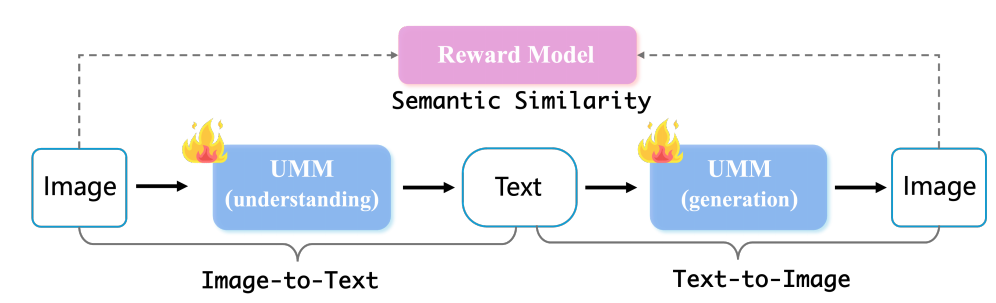
\includegraphics{images/image-0054.png}
\caption{UAE 将图像理解与图像生成串成自编码器式训练流水线}
\end{figure}

\begin{figure}[htbp]
\centering
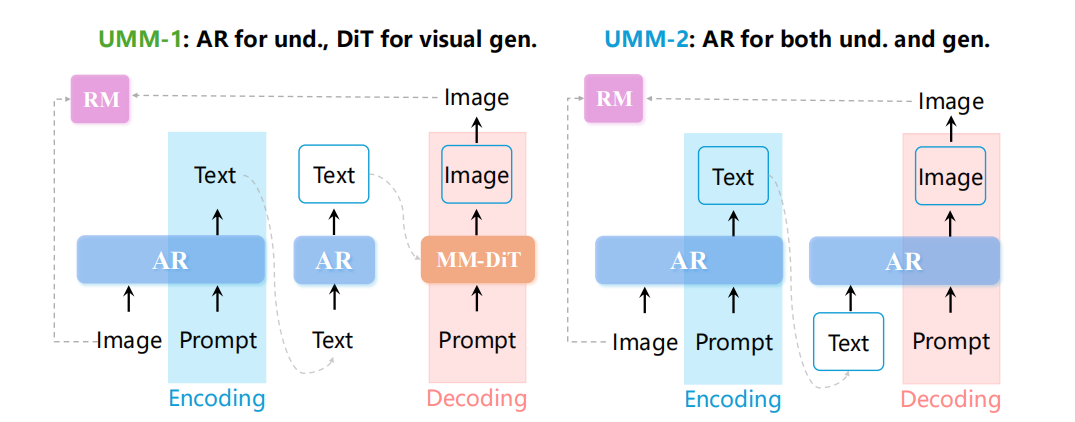
\includegraphics{images/image-0055.png}
\caption{UAE 中 UMM-1 与 UMM-2 两类统一多模态模型的编码和解码方式}
\end{figure}

\hypertarget{ux4e8cux8badux7ec3ux6d41ux7a0b}{%
\subsection{二、训练流程}\label{ux4e8cux8badux7ec3ux6d41ux7a0b}}

\hypertarget{ux4e00umm-1ux7c7bux6a21ux578b}{%
\subsubsection{（一）UMM-1类模型}\label{ux4e00umm-1ux7c7bux6a21ux578b}}

冻结Decoder（即Diffusion Transformer），将其作为RL环境的一部分，只用GRPO训练Encoder（即自回归模型）。Encoder中的ViT也要冻结，因为ViT负责把原始图像像素转化为视觉 token，是LLM的``眼睛''，一旦视觉特征在RL中发生漂移，整个系统将失去稳定基准。消融实验表明，如果对视觉编码器（ViT）或DiT也做梯度更新，RL的随机性和高方差梯度会导致生成崩溃，表现为语义信息丢失、结构坍塌、出现异常伪影等。

在训练的过程中，针对Encoder生成的每一条文本，提取其最后一个隐状态向量，通过一个投影层将其映射为扩散模型的条件输入。模型会学会在表示文段生成结束的最后一个 token中蕴含丰富的全局语义信息。

\hypertarget{ux4e8cumm-2ux7c7bux6a21ux578b}{%
\subsubsection{（二）UMM-2类模型}\label{ux4e8cumm-2ux7c7bux6a21ux578b}}

Encoder和Decoder完全相同，故同步训练。梯度（或相对优势估计）不仅会指导模型如何更好地提取语义，还会直接指导模型如何更精准地将文本翻译回视觉token。这样可以真正实现协同进化：理解能力的提升为生成提供了更密集的先验信号，而生成过程为了达到极高的还原度，反过来促使模型在统一的权重空间内完善其细粒度的视觉感知能力（例如对小目标或细微属性的捕捉）。

Encoder中的ViT也需要冻结，原因与前面所述相同。

\hypertarget{ux4e09ux4f7fux7528rlux7684ux539fux56e0ux548cux5956ux52b1ux51fdux6570}{%
\subsection{三、使用RL的原因和奖励函数}\label{ux4e09ux4f7fux7528rlux7684ux539fux56e0ux548cux5956ux52b1ux51fdux6570}}

由于``模型需要生成怎样的文本''没有可学习的Ground Truth，只通过图像生成情况好坏来评判，故这里使用强化学习中的GRPO算法，而不是监督学习或无监督学习。奖励计算方式如下：

具体操作是：使用预训练的 CLIP 模型分别提取原始输入图像 \(x\) 和重建图像 \(\tilde{x}^{(i)}\) 的视觉特征向量，并计算二者之间的余弦相似度作为单次采样的奖励值 \(\mathcal{R}\)：

\[
\mathcal{R}(x, \tilde{x}) = \cos\left(f_{\mathrm{CLIP}}(x), f_{\mathrm{CLIP}}(\tilde{x})\right)
\]

这样做有两个原因：

\begin{itemize}
\tightlist
\item
  不使用传统的像素级均方误差（MSE），是因为该框架中的``中间隐空间''是纯文本字典，文本只能保留语义级特征，例如物体、颜色和位置，无法保留光照、噪点、微小纹理等底层像素变化。如果强制用 MSE 作为奖励，算法会严重惩罚新图像和原图在底层像素上的变化，违背评估``语义一致性''的初衷。
\item
  使用 CLIP，是因为 CLIP 擅长在高维空间对齐高级语义。最大化 CLIP 相似度只要求重建图像和原图在核心属性与空间关系上吻合，这更接近``模型是否全面理解图像''的评估目标。
\end{itemize}

\hypertarget{ux53c2ux8003ux6587ux732e-200}{%
\subsection{参考文献}\label{ux53c2ux8003ux6587ux732e-200}}

\begin{itemize}
\tightlist
\item
  Yan, Z., Lin, K., Li, Z., Ye, J., Han, H., Wang, Z., Liu, H., Lin, B., Li, H., Xu, X., Xiao, X., Wang, J., Wang, H., \& Yuan, L. (2025). \href{https://arxiv.org/abs/2509.09666}{Unified Multimodal Models as Auto-Encoders}. arXiv:2509.09666.
\end{itemize}

\clearpage

\hypertarget{visionbananaux7528ux89c6ux89c9ux751fux6210ux7edfux4e00ux7406ux89e3ux4efbux52a1ux8bbaux6587}{%
\section{VisionBanana：用视觉生成统一理解任务（论文）}\label{visionbananaux7528ux89c6ux89c9ux751fux6210ux7edfux4e00ux7406ux89e3ux4efbux52a1ux8bbaux6587}}

\begin{quote}
本文是论文阅读笔记，内容代表对应论文方法或作者理解，不应直接视为领域共识或工程最佳实践。
\end{quote}

\hypertarget{ux4e00ux95eeux9898ux80ccux666f-15}{%
\subsection{一、问题背景}\label{ux4e00ux95eeux9898ux80ccux666f-15}}

目前的图像生成和图像理解还难以统一到一个模型中，实践中常常会发现二者的梯度是冲突的。但这和我们的直觉是相悖的：图像生成模型在训练时需要学会物体、场景、几何、语义、材质、空间关系等，这已经包含了对图像的理解。

对于分割、深度、法线这些视觉理解任务，过去也有人观察到生成模型偶尔能画出类似``深度图''``分割图''的东西，但这些输出格式不稳定，不能可靠解码成标准视觉任务结果，也很难拿去和专用模型公平评测。

\hypertarget{ux4e8cux6838ux5fc3ux601dux60f3-7}{%
\subsection{二、核心思想}\label{ux4e8cux6838ux5fc3ux601dux60f3-7}}

论文《Image Generators are Generalist Vision Learners》的核心贡献在于把所有视觉理解任务都重新表述成``生成一张RGB图像''，然后让图像生成器按照指令生成可解码的视觉结果。作者基于图像生成模型~Nano Banana Pro，做轻量级指令微调，得到~Vision Banana，输入原始图像+自然语言指令，输出一张RGB图像，再转换回标准视觉任务结果，例如mask、深度值、法线方向。例如，语义分割不再让模型输出类别logits，而是让模型生成一张彩色分割图：``请生成这张图的语义分割可视化图： 道路用红色，天空用蓝色，行人用黄色，背景用黑色。''模型生成RGB图后，系统根据颜色把每个像素解码成类别。这样，分割任务就被转换成了图像生成任务。

这和大语言模型的范式很像，LLM通过文本生成统一处理翻译、问答、推理、代码等任务；这篇论文则试图证明，图像生成也可以成为视觉理解任务的统一接口。分割图、深度图、法线图都可以编码成RGB图，让一个生成模型用同一种输出形式处理多种任务。Vision Banana没有为每个任务单独设计新头部、新网络或新损失，而是共享同一个生成模型，只换prompt和输出颜色编码规则。论文指出，Vision Banana在多个任务上达到或接近专用模型的水平。

\hypertarget{ux4e09ux4efbux52a1ux7c7bux522b}{%
\subsection{三、任务类别}\label{ux4e09ux4efbux52a1ux7c7bux522b}}

\hypertarget{ux4e002dux8bedux4e49ux7406ux89e3}{%
\subsubsection{（一）2D语义理解}\label{ux4e002dux8bedux4e49ux7406ux89e3}}

语义分割：给每个像素分配语义类别，例如路、人、天空、车。
实例分割：同一类别的不同物体实例要分开，例如五只狗要有五个不同mask。
指代表达分割：根据自然语言描述找出目标区域，例如``穿粉色T恤的男人''``正在伸懒腰的猫''``菜单上中英文厨师名字''。

\hypertarget{ux4e8c3dux51e0ux4f55ux7406ux89e3}{%
\subsubsection{（二）3D几何理解}\label{ux4e8c3dux51e0ux4f55ux7406ux89e3}}

单目metric depth estimation：从一张RGB图估计每个像素到相机的真实物理距离，单位是米。
surface normal estimation：估计每个像素所在表面的朝向，也就是局部3D几何方向。

\hypertarget{ux56dbux8badux7ec3ux65b9ux5f0f}{%
\subsection{四、训练方式}\label{ux56dbux8badux7ec3ux65b9ux5f0f}}

Vision Banana是在Nano Banana Pro上做轻量级指令微调。训练数据混合两部分：

原始图像生成训练数据：保持模型原本的图像生成能力。

少量视觉任务数据：教模型把视觉任务输出成指定格式的RGB图。

论文特别强调视觉任务数据比例很低，目的不是从头训练一个分割/深度模型，而是教生成器``听懂任务格式''，把它内部已有的视觉表示转成可测量输出。作者想证明的是：视觉理解能力主要来自生成式预训练，而不是来自大量任务专用微调。

\hypertarget{ux4e94ux7f16ux7801ux89c4ux5219}{%
\subsection{五、编码规则}\label{ux4e94ux7f16ux7801ux89c4ux5219}}

最简单的是分割任务。假设模型生成的图像为：

\[
G(x, y) \in [0, 255]^3
\]

其中 \(G(x, y)\) 表示像素 \((x, y)\) 的 RGB 颜色。prompt 里规定类别 \(c\) 对应颜色 \(q_c\)，那么解码时可以用最近颜色匹配：

\[
\hat{c}(x, y) = \arg\min_c \left\|G(x, y) - q_c\right\|_2
\]

意思是：对每个像素，找它生成颜色最接近哪个类别颜色，就把它归到那个类别。

实例分割稍微不同，因为实例数量事先未知，不能提前在 prompt 里指定每个实例的颜色。论文采用 per-class inference：每次只让模型分割某一类，例如``每个 garlic instance 用不同颜色表示''。模型自己给不同实例分配颜色，后处理时再根据颜色聚类，把不同颜色区域拆成不同实例。

深度估计更复杂，因为深度是实数：

\[
d \in [0, \infty)
\]

而 RGB 是有限范围：

\[
RGB \in [0, 1]^3
\]

因此作者设计了一个可逆映射，把真实深度 \(d\) 编码成 RGB 颜色。论文使用 Barron 的 power transform 先把深度压缩到 \([0, 1)\)：

\[
f(d, \lambda, c) = 1 - \left(1 - \frac{d}{\lambda c}\right)^{\lambda + 1}
\]

其中，\(d\) 是真实 metric depth，单位是米；\(\lambda\) 是形状参数，论文实验中取 \(-3\)；\(c\) 是尺度参数，论文实验中取 \(10/3\)；\(f(d,\lambda,c)\) 是归一化后的深度值，用来映射到 RGB 色彩路径上。

这样做的原因是：近处物体的深度误差通常更重要，所以映射会给近距离分配更高分辨率，远距离则被压缩。随后，论文把这个归一化深度沿 RGB 立方体边缘映射成颜色。推理时，模型生成彩色深度图，再通过反函数把颜色解码回米制深度。

表面法线更直接。法线是单位向量：

\[
\mathbf{n} = (x, y, z), \quad x, y, z \in [-1, 1]
\]

RGB 通道是 \([0, 1]\)，所以可以使用线性变换：

\[
RGB = \frac{\mathbf{n} + 1}{2}
\]

也就是：

\[
R = \frac{x + 1}{2}, \quad G = \frac{y + 1}{2}, \quad B = \frac{z + 1}{2}
\]

生成图像后再反解：

\[
\mathbf{n} = 2RGB - 1
\]

这样 RGB 图就可以表示每个像素的表面朝向。

\hypertarget{ux53c2ux8003ux6587ux732e-201}{%
\subsection{参考文献}\label{ux53c2ux8003ux6587ux732e-201}}

\begin{itemize}
\tightlist
\item
  Gabeur, V., Long, S., Peng, S., Voigtlaender, P., Sun, S., Bao, Y., Truong, K., Wang, Z., Zhou, W., Barron, J. T., Genova, K., Kannen, N., Ben, S., Li, Y., Guo, M., Yogin, S., Gu, Y., Chen, H., Wang, O., Xie, S., Zhou, H., He, K., Funkhouser, T., Alayrac, J.-B., \& Soricut, R. (2026). \href{https://arxiv.org/abs/2604.20329}{Image Generators are Generalist Vision Learners}. arXiv:2604.20329.
\end{itemize}

\clearpage

\hypertarget{uni-3darux8de8ux5c3aux5ea63dux7ed3ux6784ux7684ux7edfux4e00ux7406ux89e3ux4e0eux751fux6210ux8bbaux6587}{%
\section{Uni-3DAR：跨尺度3D结构的统一理解与生成（论文）}\label{uni-3darux8de8ux5c3aux5ea63dux7ed3ux6784ux7684ux7edfux4e00ux7406ux89e3ux4e0eux751fux6210ux8bbaux6587}}

\begin{quote}
本文是论文阅读笔记，内容代表对应论文方法或作者理解，不应直接视为领域共识或工程最佳实践。
\end{quote}

\hypertarget{ux4e00ux95eeux9898ux80ccux666f-16}{%
\subsection{一、问题背景}\label{ux4e00ux95eeux9898ux80ccux666f-16}}

长期以来，3D 结构建模在不同尺度上是割裂的：

\begin{itemize}
\tightlist
\item
  宏观与微观的壁垒：宏观模型，例如用于 3D 重建、流体力学的模型，无法直接应用于微观领域，例如蛋白质折叠、晶体生成。
\item
  任务特异性：即使在相似的尺度下，为晶体生成设计的模型也无法直接用于蛋白质折叠。这导致模型高度专业化、存在大量冗余，且无法实现数据的有效复用。
\item
  现有生成模型的局限性：主流扩散模型在微观生成中需要预先设定原子数量，而且原子类型是离散的类别分布，扩散模型难以定义完美的得分函数。
\end{itemize}

Uni-3DAR将不同尺度的3D结构用统一的通用方法表示，并统一到自回归的Next token prediction框架下，为将3D结构模态融入统一多模态理解-生成模型奠定基础。

\hypertarget{ux4e8c3dux7ed3ux6784ux8868ux793aux65b9ux6cd5}{%
\subsection{二、3D结构表示方法}\label{ux4e8c3dux7ed3ux6784ux8868ux793aux65b9ux6cd5}}

\hypertarget{ux4e00ux52a8ux6001ux7531ux7c97ux5230ux7ec6ux7684ux516bux53c9ux6811-token-ux5316}{%
\subsubsection{（一）动态由粗到细的八叉树 Token 化}\label{ux4e00ux52a8ux6001ux7531ux7c97ux5230ux7ec6ux7684ux516bux53c9ux6811-token-ux5316}}

3D 空间本质上是高度稀疏的，无论是微观分子还是宏观物体表面。如果直接使用完整的 3D 体素网格（Voxel Grid），计算量会呈指数级爆炸。Uni-3DAR 采用了基于八叉树（Octree）的无损压缩方法：

\begin{itemize}
\tightlist
\item
  空间划分：从包含整个结构的单一根节点细胞开始，递归地将空间等分为 \(2^3 = 8\) 个子细胞。
\item
  数学推导：假设根节点的边长为 \(c_0\)，则在第 \(L\) 层（深度为 \(L\)）的叶子节点边长为：
\end{itemize}

\[
c_{L-1} = \frac{c_0}{2^{L-1}}
\]

\begin{itemize}
\tightlist
\item
  自适应剪枝：只有包含实体（如原子或物体表面）的区域才会被继续划分，空的区域分支会被直接剪枝。这使得最高层最多只有 \(8^{L-1}\) 个叶子节点，而且绝大部分节点会因为稀疏性被剪去。
\end{itemize}

\hypertarget{ux4e8cux7ec6ux7c92ux5ea6ux7ed3ux6784ux8868ux793a}{%
\subsubsection{（二）细粒度结构表示}\label{ux4e8cux7ec6ux7c92ux5ea6ux7ed3ux6784ux8868ux793a}}

八叉树只能确定``哪里有东西''（占据状态），但无法描述细节。因此，在八叉树的最底层，非空叶子节点被视为 3D Patch：

\begin{itemize}
\tightlist
\item
  微观尺度（如分子）：将 Patch 大小设置为 \(c_{L-1}=0.24\,\mathrm{\mathring{A}}\)，确保每个 Patch 最多只包含一个原子。Token 包含原子类型 \(t_i\) 和在细胞内的精确连续坐标 \(e_i=(e_i^0,e_i^1,e_i^2)\)。坐标通过分辨率 \(c_r=0.01\,\mathrm{\mathring{A}}\) 离散化为 \(N_p=c_{L-1}/c_r\) 个区间。
\item
  宏观尺度：使用 VQ-VAE 将体素块量化为离散的字典 Token。
\end{itemize}

\hypertarget{ux4e09ux6838ux5fc3ux539fux7406}{%
\subsection{三、核心原理}\label{ux4e09ux6838ux5fc3ux539fux7406}}

第一阶段是动态展开``脚手架''，也就是预测空间占据。模型并不是一上来就直接预测原子，而是从宏观到微观，逐层预测空间的占据情况：

\begin{enumerate}
\def\labelenumi{\arabic{enumi}.}
\tightlist
\item
  模型一开始面对的是一个包含整个分子的巨大``根节点''细胞。
\item
  模型预测这个大细胞的 8 个子区块中哪几个有东西，这相当于前面提到的两层子树压缩的 256 分类任务。
\item
  对于预测``有东西''的子区块，模型继续往下细分，直到到达最底层（第 \(L-1\) 层，也就是边长为 \(0.24\,\mathrm{\mathring{A}}\) 的微小细胞）。
\item
  关键点在于，这一层层的细胞是模型自己刚刚自回归预测出来的，所以当它预测出``最底层的某个微小细胞 A 被占据''时，细胞 A 的中心坐标对模型来说已经是绝对已知的。
\end{enumerate}

第二阶段是在已知位置放置 \texttt{MASK} Token 并预测``细节''，也就是填补内容。此时，模型已经在空间中划分出一系列已知坐标、微小且被占据的``叶子细胞''：

\begin{enumerate}
\def\labelenumi{\arabic{enumi}.}
\tightlist
\item
  放置掩码：模型在刚才推导出的细胞 A 的中心坐标处，放置一个 \texttt{MASK} Token。因此，这个 \texttt{MASK} Token 的位置是已知的，它代表``这个极其微小的空间块''。
\item
  预测对象：既然位置已经固定在细胞 A，模型接下来要预测的内容就是这个细胞里装的是什么，包括类型 \(t_i\)，以及原子在细胞 A 内部的具体相对偏移量 \(e_i\)。
\end{enumerate}

为什么要这么做：

如果让模型直接在虚空中预测一个原子的绝对坐标，例如 \(x = 12.34, y = 5.67, z = 8.90\)，就相当于让模型``盲猜''，没有任何空间参照系。这在自回归模型中表现很差，因为上一个生成的原子和下一个生成的原子在空间上可能毫无规律可言。

Uni-3DAR 通过 MNTP（掩码下个 Token 预测）配合八叉树，把``盲猜''变成一道``填空题''：

\begin{itemize}
\tightlist
\item
  传统方式问的是：``下一个原子是什么？它在宇宙中的哪里？''这很难。
\item
  Uni-3DAR 的方式问的是：``根据刚才生成的空间轮廓，我知道坐标 \((x,y,z)\) 这里的微小细胞里一定有个东西，也就是已知位置的 \texttt{MASK} Token。请告诉我，它具体是什么原子？在这个微小细胞的哪个精确角落？''这大幅降低了预测难度。
\end{itemize}

\hypertarget{ux56dbux63a8ux7406ux5de5ux4f5cux6d41}{%
\subsection{四、推理工作流}\label{ux56dbux63a8ux7406ux5de5ux4f5cux6d41}}

推理时可以理解为以下循环：

\begin{itemize}
\tightlist
\item
  第 0 步（起点）：系统在 3D 宇宙中心放置一个代表最高层（Root）的 \texttt{MASK} Token，位置绝对已知。
\item
  第 1 步（预测第 0 层）：模型看着这个 \texttt{MASK} Token，结合条件（例如分子化学式），预测出它的内容，例如 \texttt{10000001}（假设转换为十进制是 129）。
\item
  第 2 步（几何推导位置）：系统读取 \texttt{10000001}，立刻知道这个大空间的第 1 号角落和第 8 号角落有东西。系统随即通过几何公式计算出这两个子角落的精确中心坐标。
\item
  第 3 步（放置新的 \texttt{MASK} Token）：系统在刚刚算出的两个精确坐标处，放置两个属于第 1 层的 \texttt{MASK} Token。
\item
  第 4 步（预测第 1 层）：模型再去预测这两个新 \texttt{MASK} Token 的内容（0 到 255）。
\item
  循环往复：预测内容、解码出子节点占据情况、算出子节点确切坐标、在新坐标放置 \texttt{MASK} Token、继续预测新内容。
\item
  终局（到达最底层）：当这个过程循环到预设的八叉树最底层，例如第 6 层、细胞边长 \(0.24\,\mathrm{\mathring{A}}\) 时，系统放置的 \texttt{MASK} Token 就不再是 0 到 255 的分类任务，而是切换成原子级预测头。模型在这个微小细胞的 \texttt{MASK} Token 处，预测具体的原子类型（碳、氢、氧等）和在细胞内的微调坐标 \(e_i\)。
\end{itemize}

\hypertarget{ux4e94ux8badux7ec3ux65b9ux6cd5}{%
\subsection{五、训练方法}\label{ux4e94ux8badux7ec3ux65b9ux6cd5}}

\hypertarget{ux4e00ux6574ux4f53ux8badux7ec3ux8303ux5f0fteacher-forcing-ux4e0bux7684ux586bux7a7aux9898}{%
\subsubsection{（一）整体训练范式：Teacher Forcing 下的``填空题''}\label{ux4e00ux6574ux4f53ux8badux7ec3ux8303ux5f0fteacher-forcing-ux4e0bux7684ux586bux7a7aux9898}}

和 GPT 等大语言模型的训练方式类似，Uni-3DAR 在训练时采用 Teacher Forcing（教师强制）机制。在训练阶段，模型其实是在``看着正确答案''学习。系统会将真实的 3D 结构完整地转换为八叉树加原子的 Token 序列，并在所有应该预测的位置打上 \texttt{MASK} Token。模型需要同时对序列中的所有 \texttt{MASK} Token 进行预测，计算预测分布与真实内容之间的差距（Loss），然后反向传播更新权重。

\hypertarget{ux4e8cux5b8fux89c2ux9aa8ux67b6ux7684ux8badux7ec3ux516bux53c9ux6811-token-ux9884ux6d4b}{%
\subsubsection{（二）宏观骨架的训练：八叉树 Token 预测}\label{ux4e8cux5b8fux89c2ux9aa8ux67b6ux7684ux8badux7ec3ux516bux53c9ux6811-token-ux9884ux6d4b}}

对于八叉树中间节点的 \texttt{MASK} Token，模型的训练目标是预测它的 8 个子节点是否存在：

\begin{itemize}
\tightlist
\item
  损失函数：标准的 256 分类交叉熵损失（Cross-Entropy Loss）。
\item
  这一阶段让模型学习如何根据化学式或整体轮廓，正确地``开疆拓土''。
\end{itemize}

\hypertarget{ux4e09ux5e95ux90e8ux539fux5b50ux7684ux8badux7ec3ux7ec6ux8282ux5faeux89c2ux7ec6ux7c92ux5ea6ux9884ux6d4b}{%
\subsubsection{（三）底部原子的训练细节：微观细粒度预测}\label{ux4e09ux5e95ux90e8ux539fux5b50ux7684ux8badux7ec3ux7ec6ux8282ux5faeux89c2ux7ec6ux7c92ux5ea6ux9884ux6d4b}}

当序列推进到八叉树的最底层，也就是叶子节点细胞、边长 \(0.24\,\mathrm{\mathring{A}}\) 时，这里的 \texttt{MASK} Token 对应的真实内容是一个具体原子。对这个底层 \texttt{MASK} Token 的训练被拆解为更细的步骤：

\begin{enumerate}
\def\labelenumi{\arabic{enumi}.}
\tightlist
\item
  预测原子类型 \(t_i\)：模型首先看着底层 \texttt{MASK} Token，预测这个微小细胞里装的是什么原子，例如碳、氢、氧等。这仍然是标准分类任务，使用交叉熵损失。
\item
  预测细胞内连续坐标 \(e_i\)：确定原子类型后，还要确定它在这个极小细胞内的精确相对位置。因为坐标是连续值，直接回归比较难，Uni-3DAR 采用更像语言模型的做法：先将连续坐标按照 \(0.01\,\mathrm{\mathring{A}}\) 的高分辨率离散化，切分成整数索引 \(0\) 到 \(N_p-1\)；再采用内部自回归方式预测坐标，先预测 \(x\) 坐标分类概率，再用真实的 \(x\) 坐标作为条件预测 \(y\) 坐标，最后用真实的 \(x,y\) 坐标作为条件预测 \(z\) 坐标。
\end{enumerate}

\(x,y,z\) 的预测也被视为离散分类任务，会产生 3 个交叉熵损失。论文也提到，可以使用 Token 级别的 Diffusion 扩散损失来预测连续坐标，但由于自回归分类的方式更高效且效果相当，所以默认采用自回归预测坐标。

这样，就可以将3D结构生成统一到Next token prediction的框架下。

\hypertarget{ux56dbux635fux5931ux7684ux6c47ux805a}{%
\subsubsection{（四）损失的汇聚}\label{ux56dbux635fux5931ux7684ux6c47ux805a}}

在一次训练迭代中，模型实际会计算整个序列中所有掩码的损失之和：

\textbf{总损失 = 所有八叉树节点的 256 分类 Loss + 所有底部原子的类型 Loss + 所有底部原子的 X、Y、Z 坐标 Loss。}

\hypertarget{ux53c2ux8003ux6587ux732e-202}{%
\subsection{参考文献}\label{ux53c2ux8003ux6587ux732e-202}}

\begin{itemize}
\tightlist
\item
  Lu, S., Lin, H., Yao, L., Gao, Z., Ji, X., E, W., Zhang, L., \& Ke, G. (2025). \href{https://arxiv.org/abs/2503.16278}{Uni-3DAR: Unified 3D Generation and Understanding via Autoregression on Compressed Spatial Tokens}. arXiv:2503.16278.
\end{itemize}

\clearpage
